\documentclass[fleqn,10pt,c]{beamer}

\usepackage[english]{babel}
\usepackage[utf8]{inputenc}
\usepackage[T1]{fontenc}


\usepackage{amsmath} % Maths
\usepackage{amsfonts} % Maths
\usepackage{amssymb} % Maths
\usepackage{stmaryrd} % Maths (crochets doubles)

%\usepackage{listings} % Mise en forme du code (pour Hoare) ## À REVOIR ###
%\usepackage{ifthen} % Structures If Then Else
\usepackage{theorem} % Styles supplémentaires pour théorèmes
\usepackage{url}
\usepackage{array}  % Tableaux évolués
\usepackage{multirow}  % Pour des colonnes sur plusieurs lignes

%\usepackage{enumerate} % Changer les puces des listes d'énumération
%\usepackage{setspace} % Changer les interlignes

%\usepackage{subfig} % Créer des sous-figures
%\usepackage{graphicx} % Importer des images

\usepackage{ulem}  % Pour l'attribut barré

\usepackage{comment}

% Police
\usepackage{lmodern}
%\usepackage{libertine}

\usepackage{tikz}
\usepackage{tkz-tab}
\newdimen\pgfex
\newdimen\pgfem
\usetikzlibrary{arrows,shapes,shadows,scopes}
\usetikzlibrary{positioning}
\usetikzlibrary{matrix}
\usetikzlibrary{decorations.text}
\usetikzlibrary{decorations.pathmorphing}

%il faudra rajouter des macros
% Macros relatives à la traduction de PH avec arcs neutralisants vers PH à k-priorités fixes

% Macros générales
%\newcommand{\ie}{\textit{i.e.} }
\newcommand{\segm}[2]{\llbracket #1; #2 \rrbracket}
%\newcommand{\f}[1]{\mathsf{#1}}

% Notations générales pour PH
\newcommand{\PH}{\mathcal{PH}}
%\newcommand{\PHs}{\mathcal{S}}
\newcommand{\PHs}{\Sigma}
%\newcommand{\PHp}{\mathcal{P}}
\newcommand{\PHp}{\textcolor{red}{\mathcal{P}}}
%\newcommand{\PHproc}{\mathcal{P}}
\newcommand{\PHproc}{\mathbf{Proc}}
\newcommand{\Proc}{\PHproc}
\newcommand{\PHh}{\mathcal{H}}
\newcommand{\PHa}{\PHh}
%\newcommand{\PHa}{\mathcal{A}}
\newcommand{\PHl}{\mathcal{L}}
\newcommand{\PHn}{\mathcal{N}}

\newcommand{\PHhitter}{\mathsf{hitter}}
\newcommand{\PHtarget}{\mathsf{target}}
\newcommand{\PHbounce}{\mathsf{bounce}}
%\newcommand{\PHsort}{\Sigma}
\newcommand{\PHsort}{\PHs}

%\newcommand{\PHfrappeur}{\mathsf{frappeur}}
%\newcommand{\PHcible}{\mathsf{cible}}
%\newcommand{\PHbond}{\mathsf{bond}}
%\newcommand{\PHsorte}{\mathsf{sorte}}
%\newcommand{\PHbloquant}{\mathsf{bloquante}}
%\newcommand{\PHbloque}{\mathsf{bloquee}}

%\newcommand{\PHfrappeR}{\textcolor{red}{\rightarrow}}
%\newcommand{\PHmonte}{\textcolor{red}{\Rsh}}

\newcommand{\PHhitA}{\rightarrow}
\newcommand{\PHhitB}{\Rsh}
%\newcommand{\PHfrappe}[3]{\mbox{$#1\PHhitA#2\PHhitB#3$}}
%\newcommand{\PHfrappebond}[2]{\mbox{$#1\PHhitB#2$}}
\newcommand{\PHhit}[3]{#1\PHhitA#2\PHhitB#3}
\newcommand{\PHfrappe}{\PHhit}
\newcommand{\PHhbounce}[2]{#1\PHhitB#2}
\newcommand{\PHobj}[2]{\mbox{$#1\PHhitB^*\!#2$}}
\newcommand{\PHobjectif}{\PHobj}
\newcommand{\PHconcat}{::}
%\newcommand{\PHneutralise}{\rtimes}

\def\PHget#1#2{{#1[#2]}}
%\newcommand{\PHchange}[2]{#1\langle #2 \rangle}
%\newcommand{\PHchange}[2]{(#1 \Lleftarrow #2)}
%\newcommand{\PHarcn}[2]{\mbox{$#1\PHneutralise#2$}}
\newcommand{\PHplay}{\cdot}

\newcommand{\PHstate}[1]{\mbox{$\langle #1 \rangle$}}
\newcommand{\PHetat}{\PHstate}

\def\supp{\mathsf{support}}
\def\first{\mathsf{first}}
\def\last{\mathsf{last}}

\def\DNtrans{\rightarrow_{ADN}}
\def\DNdef{(\mathbb F, \langle f^1, \dots, f^n\rangle)}
\def\DNdep{\mathsf{dep}}
\def\PHPtrans{\rightarrow_{PH}}
\def\get#1#2{#1[{#2}]}
\def\encodeF#1{\mathbf{#1}}
\def\toPH{\encodeF{PH}}
\def\card#1{|#1|}
\def\decode#1{\llbracket#1\rrbracket}
\def\encode#1{\llparenthesis#1\rrparenthesis}
\def\Hits{\PHa}
\def\hit{\PHhit}
\def\play{\cdot}

\def\Pint{\textsc{PINT}}


%rajout pour les labels sur les arcs 
\tikzstyle{labelprio}=[circle, fill=blue!30, inner sep=0pt, minimum size=13pt]
\tikzstyle{labelprio1}=[labelprio]
\tikzstyle{labelprio2}=[labelprio, fill=red!60]
\tikzstyle{labelprio3}=[labelprio, fill=orange!50]
\tikzstyle{labelprio4}=[labelprio, fill=brown!50]




\usepackage{ifthen}

\newcommand{\currentScope}{}
\newcommand{\currentSort}{}
\newcommand{\currentSortLabel}{}
\newcommand{\currentAlign}{}
\newcommand{\currentSize}{}

\newcounter{la}
\newcommand{\TSetSortLabel}[2]{
  \expandafter\repcommand\expandafter{\csname TUserSort@#1\endcsname}{#2}
}
\newcommand{\TSort}[4]{
  \renewcommand{\currentScope}{#1}
  \renewcommand{\currentSort}{#2}
  \renewcommand{\currentSize}{#3}
  \renewcommand{\currentAlign}{#4}
  \ifcsname TUserSort@\currentSort\endcsname
    \renewcommand{\currentSortLabel}{\csname TUserSort@\currentSort\endcsname}
  \else
    \renewcommand{\currentSortLabel}{\currentSort}
  \fi
  \begin{scope}[shift={\currentScope}]
  \ifthenelse{\equal{\currentAlign}{l}}{
    \filldraw[process box] (-0.5,-0.5) rectangle (0.5,\currentSize-0.5);
    \node[sort] at (-0.2,\currentSize-0.4) {\currentSortLabel};
   }{\ifthenelse{\equal{\currentAlign}{r}}{
     \filldraw[process box] (-0.5,-0.5) rectangle (0.5,\currentSize-0.5);
     \node[sort] at (0.2,\currentSize-0.4) {\currentSortLabel};
   }{
    \filldraw[process box] (-0.5,-0.5) rectangle (\currentSize-0.5,0.5);
    \ifthenelse{\equal{\currentAlign}{t}}{
      \node[sort,anchor=east] at (-0.3,0.2) {\currentSortLabel};
    }{
      \node[sort] at (-0.6,-0.2) {\currentSortLabel};
    }
   }}
  \setcounter{la}{\currentSize}
  \addtocounter{la}{-1}
  \foreach \i in {0,...,\value{la}} {
    \TProc{\i}
  }
  \end{scope}
}

\newcommand{\TTickProc}[2]{ % pos, label
  \ifthenelse{\equal{\currentAlign}{l}}{
    \draw[tick] (-0.6,#1) -- (-0.4,#1);
    \node[tick label, anchor=east] at (-0.55,#1) {#2};
   }{\ifthenelse{\equal{\currentAlign}{r}}{
    \draw[tick] (0.6,#1) -- (0.4,#1);
    \node[tick label, anchor=west] at (0.55,#1) {#2};
   }{
    \ifthenelse{\equal{\currentAlign}{t}}{
      \draw[tick] (#1,0.6) -- (#1,0.4);
      \node[tick label, anchor=south] at (#1,0.55) {#2};
    }{
      \draw[tick] (#1,-0.6) -- (#1,-0.4);
      \node[tick label, anchor=north] at (#1,-0.55) {#2};
    }
   }}
}
\newcommand{\TSetTick}[3]{
  \expandafter\repcommand\expandafter{\csname TUserTick@#1_#2\endcsname}{#3}
}

\newcommand{\myProc}[3]{
  \ifcsname TUserTick@\currentSort_#1\endcsname
    \TTickProc{#1}{\csname TUserTick@\currentSort_#1\endcsname}
  \else
    \TTickProc{#1}{#1}
  \fi
  \ifthenelse{\equal{\currentAlign}{l}\or\equal{\currentAlign}{r}}{
    \node[#2] (\currentSort_#1) at (0,#1) {#3};
  }{
    \node[#2] (\currentSort_#1) at (#1,0) {#3};
  }
}
\newcommand{\TSetProcStyle}[2]{
  \expandafter\repcommand\expandafter{\csname TUserProcStyle@#1\endcsname}{#2}
}
\newcommand{\TProc}[1]{
  \ifcsname TUserProcStyle@\currentSort_#1\endcsname
    \myProc{#1}{\csname TUserProcStyle@\currentSort_#1\endcsname}{}
  \else
    \myProc{#1}{process}{}
  \fi
}

\newcommand{\repcommand}[2]{
  \providecommand{#1}{#2}
  \renewcommand{#1}{#2}
}
\newcommand{\THit}[5]{
  \path[hit] (#1) edge[#2] (#3#4);
  \expandafter\repcommand\expandafter{\csname TBounce@#3@#5\endcsname}{#4}
}
\newcommand{\TBounce}[4]{
  (#1\csname TBounce@#1@#3\endcsname) edge[#2] (#3#4)
}

%\newcommand{\TState}[1]{
%  \foreach \proc in {#1} {
%    \node[current process] (\proc) at (\proc.center) {};
%  }
%}

\newcommand{\TState}[2]{
  \foreach \proc in {#2} {
        \only<#1>{ \node[current process] (\proc) at (\proc.center) {}; }
  };
}

\newdimen\pgfex
\newdimen\pgfem
\usetikzlibrary{arrows,shapes,shadows,scopes}
\usetikzlibrary{positioning}
\usetikzlibrary{matrix}
\usetikzlibrary{decorations.text}
\usetikzlibrary{decorations.pathmorphing}

\usetikzlibrary{arrows,shapes}

\definecolor{lightgray}{rgb}{0.8,0.8,0.8}
\definecolor{lightgrey}{rgb}{0.8,0.8,0.8}

\definecolor{lightred}{rgb}{1,0.8,0.8}
\definecolor{lightgreen}{rgb}{0.7,1,0.7}
\definecolor{darkgreen}{rgb}{0,0.5,0}
\definecolor{darkblue}{rgb}{0,0,0.5}
\definecolor{darkyellow}{rgb}{0.5,0.5,0}
\definecolor{lightyellow}{rgb}{1,1,0.6}
\definecolor{darkcyan}{rgb}{0,0.6,0.6}
\definecolor{lightcyan}{rgb}{0.6,1,1}
\definecolor{darkorange}{rgb}{0.8,0.2,0}
\definecolor{notsodarkred}{rgb}{0.8,0,0}

\definecolor{notsodarkgreen}{rgb}{0,0.7,0}

%\definecolor{coloract}{rgb}{0,1,0}
%\definecolor{colorinh}{rgb}{1,0,0}
\colorlet{coloract}{darkgreen}
\colorlet{colorinh}{red}
\colorlet{coloractgray}{lightgreen}
\colorlet{colorinhgray}{lightred}
\colorlet{colorinf}{darkgray}
\colorlet{coloractgray}{lightgreen}
\colorlet{colorinhgray}{lightred}

\colorlet{colorgray}{lightgray}
\colorlet{colorhl}{blue}


\tikzstyle{boxed ph}=[]
\tikzstyle{sort}=[fill=lightgray, rounded corners, draw=black]
\tikzstyle{process}=[circle,draw,minimum size=15pt,fill=white,font=\footnotesize,inner sep=1pt]
%\tikzstyle{black process}=[process, draw=blue, fill=red,text=black,font=\bfseries]
\tikzstyle{gray process}=[process, draw=black, fill=lightgray]
\tikzstyle{highlighted process}=[current process, fill=gray]
\tikzstyle{process box}=[fill=none,draw=black,rounded corners]
%\tikzstyle{current process}=[process, draw=black, fill=lightgray]
\tikzstyle{current process}=[process,fill=blue]
\tikzstyle{hl process}=[process,fill=blue!30]
\tikzstyle{tick label}=[font=\footnotesize]
\tikzstyle{tick}=[densely dotted] %-
\tikzstyle{hit}=[->,>=angle 45]
\tikzstyle{selfhit}=[min distance=50pt,curve to]
\tikzstyle{bounce}=[densely dotted,>=stealth',->]
\tikzstyle{ulhit}=[draw=lightgray,fill=lightgray]
\tikzstyle{pulhit}=[fill=lightgray]
\tikzstyle{bulhit}=[draw=lightgray]
\tikzstyle{hl}=[very thick,colorhl]
\tikzstyle{hlb}=[very thick]
\tikzstyle{hlhit}=[hl]
%\tikzstyle{hl2}=[hl]
%\tikzstyle{nohl}=[font=\normalfont,thin]

\tikzstyle{update}=[draw,->,dashed,shorten >=.7cm,shorten <=.7cm]

\tikzstyle{unprio}=[draw,thin]%[double]
%\tikzstyle{prio}=[draw,thick,-stealth]%[double]
\tikzstyle{prio}=[draw,-stealth,double]

\tikzstyle{hitless graph}=[every edge/.style={draw=red,-}]

\tikzstyle{aS}=[every edge/.style={draw,->,>=stealth}]
\tikzstyle{Asol}=[draw,circle,minimum size=5pt,inner sep=0,node distance=1cm]
\tikzstyle{Aproc}=[draw,node distance=1.2cm]
\tikzstyle{Aobj}=[node distance=1.5cm]
\tikzstyle{Anos}=[font=\Large]

\tikzstyle{AsolPrio}=[Asol,double]
\tikzstyle{AprocPrio}=[Aproc,double]
\tikzstyle{aSPrio}=[aS,double]

\colorlet{colorhlwarn}{notsodarkred}
\colorlet{colorhlwarnbg}{lightred}
\tikzstyle{Ahl}=[very thick,fill=colorhlwarnbg,draw=colorhlwarn,text=colorhlwarn]
\tikzstyle{Ahledge}=[very thick,double=colorhlwarnbg,draw=colorhlwarn,color=colorhlwarn]
\tikzstyle{Aex}=[thick,draw=couleurex,fill=couleurex!20]
\tikzstyle{Aexedge}=[very thick,draw=couleurex,color=couleurex]


% Figure de résumé des liens entre les formalismes
\tikzstyle{equiv-externe}=[thick, rounded corners, draw=gray, fill=gray!10, align=center,
  inner sep=8]
  
\tikzstyle{local transitions}=[->,>=latex',thick,bend left=30,
                 		every node/.style={fill=white,inner sep=1pt,outer sep=1pt}]
\tikzstyle{reach}=[fill=lightgray,ellipse]




%\definecolor{darkred}{rgb}{0.5,0,0}



\tikzstyle{adn}=[every node/.style={circle,draw=black,outer sep=2pt,minimum
                size=15pt,text=black}, node distance=1.5cm, ->]
%\tikzstyle{inh}=[>=|,-|,draw=colorinh,thick, text=black,label]
%\tikzstyle{act}=[->,>=triangle 60,draw=coloract,thick,color=coloract]
%\tikzstyle{inhgray}=[>=|,-|,draw=colorinhgray,thick, text=black,label]
%\tikzstyle{actgray}=[->,>=triangle 60,draw=coloractgray,thick,color=coloractgray]
%\tikzstyle{inf}=[->,draw=colorinf,thick,color=colorinf]
%\tikzstyle{elabel}=[fill=none, above=-1pt, sloped,text=black, minimum size=10pt, outer sep=0, font=\scriptsize,draw=none]
\tikzstyle{elabel}=[fill=none,text=black, above=-2pt,%sloped,
minimum size=10pt, outer sep=0, font=\scriptsize, draw=none]
%\tikzstyle{elabel}=[]




% procedure, abstractions and dependencies
\newcommand{\abstr}[1]{#1^\wedge}%\text{\textasciicircum}}
\def\BS{\mathbf{BS}}
\def\aBS{\abstr{\BS}}
\def\abeta{\abstr{\beta}}
\def\aZ{\abstr{\zeta}}
\def\aY{\abstr{\xi}}

\def\beforeproc{\vartriangleleft}

\def\powerset{\wp}

\def\Sce{\mathbf{Sce}}
\def\OS{\mathbf{OS}}
\def\Obj{\mathbf{Obj}}
%\def\Proc{\mathbf{Proc}}
%\def\Sol{\mathbf{Sol}}
\newcommand{\Sol}{\mathbf{Sol}}

\usepackage{galois}
\newcommand{\theOSabstr}{toOS}
\newcommand{\OSabstr}[1]{\theOSabstr(#1)}
\newcommand{\theOSconcr}{toSce}
\newcommand{\OSconcr}[1]{\theOSconcr(#1)}

% \def\gO{\mathbb{O}}
% \def\gS{\mathbb{S}}
\def\aS{\mathcal{A}}
\def\Req{\mathrm{Req}}
%\def\Sol{\mathrm{Sol}}
\def\Cont{\mathrm{Cont}}
\def\cBS{\BS_\ctx}
\def\caBS{\aBS_\ctx}
\def\caS{\aS_\ctx}
\def\cSol{\Sol_\ctx}
\def\cReq{\Req_\ctx}
\def\cCont{\Cont_\ctx}

\def\any{\star}

% \def\gProc{\mathrm{maxPROC}}
\def\mCtx{\mathrm{maxCtx}}

\def\procs{\f{procs}}
\def\objs{\f{objs}}
\def\sat#1{\lceil #1\rceil}

\def\gCont{\f{maxCont}}
\def\lCont{\f{minCont}}
\def\lProc{\f{minProc}}
\def\gProc{\f{maxProc}}

\def\join{\oplus}
\def\concat{\!::\!}
\def\emptyseq{\varepsilon}
\def\ltw{\preccurlyeq_{\OS}}
\def\indexes#1{\mathbb{I}^{#1}}
%\def\indexes#1{\{1..|#1|\}}
\def\supp{\f{support}}
\def\w{\omega}
\def\W{\Omega}
\def\ctx{\varsigma}
\def\Ctx{\mathbf{Ctx}}
\def\mconcr{\gamma}
\def\concr{\mconcr_\ctx}
\def\obj#1#2{{#1\!\Rsh^*\!\!#2}}
\def\objp#1#2#3{\obj{{#1}_{#2}}{{#1}_{#3}}}
\def\A{\mathcal{A}}
\def\cwA{\A_\ctx^\w}
\def\cwReq{\Req_\ctx^\w}
\def\cwSol{\Sol_\ctx^\w}
\def\cwCont{\Cont_\ctx^\w}
\def\gCtx{\f{maxCtx}}
\def\endCtx{\f{endCtx}}
\def\ceil{\f{end}}

%\def\lfp{\mathrm{lfp}\;}
%\def\mlfp#1{\mathrm{lfp}\{#1\}\;}
\newcommand{\lfp}[3]{\mathbf{lfp}\{#1\}\left(#2\mapsto#3\right)}
\def\maxobjs{{\f{maxobjs}}}
\def\maxprocs{{\f{maxprocs}_\ctx}}
\def\objends{{\f{ends}}}

\def\ra{\rho}
\def\rb{\rho^\wedge}
\def\rc{\widetilde{\rho}}
\def\interleave{\f{interleave}}

\def\join{\concat}

\def\procs{\mathsf{procs}}
%\def\allprocs{\mathsf{allProcs}}
\def\allprocs{\procs}
%\def\pfp{\mathsf{pfp}}
\def\pfp{\mathsf{lst}}
\def\pfpprocs{\mathsf{pfpProcs}}
\def\bounceprocs{\mathsf{bounceProcs}}
\def\newprocs{\mathsf{newProcs}}

\def\aB{\mathcal{B}}
\def\sat#1{\lceil #1\rceil}
\def\cwB{\sat{\aB_\ctx^\w}}
\def\mycwB#1#2{\sat{\aB_{#1}^{#2}}}
\def\Bsol{\sat{\Sol^\w_\ctx}}
\def\Breq{\sat{\Req^\w_\ctx}}
\def\Bcont{\sat{\Cont^\w_\ctx}}

\def\myB{\aB^\w_\ctx}
\def\mysol{\overline{\Sol^\w_\ctx}}
\def\myreq{\overline{\Req^\w_\ctx}}
\def\mycont{\overline{\Cont^\w_\ctx}}

\begin{comment}
\def\PrioCont{\textcolor{red}{\mathrm{PrioCont}}}
\def\mypriocont{\overline{\PrioCont^\w_\ctx}}
\def\cwPrioCont{\PrioCont_\ctx^\w}
\def\Bpriocont{\sat{\PrioCont^\w_\ctx}}
\def\Sat{\PrioCont}
\def\mysat{\overline{\Sat^\w_\ctx}}
\def\cwSat{\Sat_\ctx^\w}
\def\Bsat{\sat{\Sat^\w_\ctx}}

\def\ReqSolPrio{\textcolor{blue}{\mathrm{ReqSolPrio}}}
\def\RSP{\ReqSolPrio}
\def\myrsp{\overline{\RSP^\w_\ctx}}
\def\cwRSP{\RSP_\ctx^\w}
\def\Brsp{\sat{\RSP^\w_\ctx}}
\end{comment}

\newcommand{\csState}{\mathsf{procState}}

\newcommand{\V}{V}
\newcommand{\E}{E}
\newcommand{\cwV}{\V_\ctx^\w}
\newcommand{\cwE}{\E_\ctx^\w}
%\newcommand{\VProc}{\textcolor{red}{\V_\PHproc}}
%\newcommand{\VObj}{\textcolor{red}{\V_\Obj}}
%\newcommand{\VSol}{\V_{Sol}}
%\newcommand{\VSol}{\textcolor{red}{\V_{\Sol}}}
\newcommand{\VProc}{\V \cap \PHproc}
\newcommand{\VObj}{\V \cap \Obj}
\newcommand{\VSol}{\V \cap \Sol}

\def\Bv{\sat{\cwV}}
\def\Be{\sat{\cwE}}
\def\BvProc{\textcolor{red}{\sat{\cwV}^\PHproc}}
\def\BvObj{\textcolor{red}{\sat{\cwV}^\Obj}}
%\def\BvSol{\sat{\cwV}^{Sol}}
\def\BvSol{\textcolor{red}{\sat{\cwV}^{\Sol}}}

\newcommand{\Bee}[2]{\Be^{#1}_{#2}}

%\def\mlfp#1{\f{pppf}\{#1\}}

\def\PHobjp#1#2#3{\PHobj{{#1}_{#2}}{{#1}_{#3}}}
\def\Obj{\mathbf{Obj}}
\def\powerset{\wp}
\def\gCont{\f{maxCont}}

\def\muconcr{\ell}
\def\uconcr{\muconcr_\ctx}

\begin{comment}
%\newcommand{\abstr}[1]{#1^\wedge}%\text{\textasciicircum}}
%\def\priomax{\mathsf{prio}_{max}}
\def\procs{\mathsf{procs}}
\def\allprocs{\mathsf{allProcs}}
\def\pfp{\mathsf{pfp}}
\def\pfpprocs{\mathsf{pfpProcs}}
%
\def\ctx{\varsigma}
\def\w{\omega}
%\def\aBS{\abstr{\BS}}
%
\def\Req{\mathrm{Req}}
\def\Sol{\mathrm{Sol}}
\def\Cont{\mathrm{Cont}}
\def\A{\mathcal{A}}
\def\cwA{\A_\ctx^\w}
\def\cwReq{\Req_\ctx^\w}
\def\cwSol{\Sol_\ctx^\w}
\def\cwCont{\Cont_\ctx^\w}
%
%
%
\end{comment}
\newcounter{imageZoom}
\newcounter{imageZoomp}
 
\usetikzlibrary{positioning}
\usetikzlibrary{calc}
 
\newcommand{\zoomZero}[2][]{
	\setcounter{imageZoom}{1}
	\draw (0,0) node[anchor=south west,inner sep=0] (image\theimageZoom) { 
  			#2
  	 	};
}
 
\newcommand{\zoomIn}[4][below]{
 	\refstepcounter{imageZoom}
 	\setcounter{imageZoomp}{\value{imageZoom}}
 	\addtocounter{imageZoomp}{-1}
	\begin{scope}[shift=(image\theimageZoomp.south west),x={(image\theimageZoomp.south east)},y={(image\theimageZoomp.north west)}]
		%\draw [step=0.05,gray,very thin] (0,0) grid (1,1);
		\node[inner sep=0,anchor=center] (rectanglebg\theimageZoomp) at (#3){};
		\node[inner sep=0,anchor=center] (rectanglehd\theimageZoomp) at ($(rectanglebg\theimageZoomp)+(#4)$){};
		\node[inner sep=0,anchor=center] (rectanglebd\theimageZoomp) at (rectanglehd\theimageZoomp |- rectanglebg\theimageZoomp){};
		\node[inner sep=0,anchor=center] (rectanglehg\theimageZoomp) at (rectanglehd\theimageZoomp -| rectanglebg\theimageZoomp){};
		\draw (#3) rectangle +(#4);
 	\end{scope}
 	\draw (0,0) node[anchor=north west,inner sep=0,#1=of image\theimageZoomp] (image\theimageZoom) {
		\phantom{#2}
	};
	\draw  (rectanglebg\theimageZoomp.center) -- (image\theimageZoom.south west);		
	\draw  (rectanglebd\theimageZoomp.center) -- (image\theimageZoom.south east);		
	\draw  (rectanglehd\theimageZoomp.center) -- (image\theimageZoom.north east);		
	\draw  (rectanglehg\theimageZoomp.center) -- (image\theimageZoom.north west);
	\draw (0,0) node[anchor=north west,inner sep=0,#1=of image\theimageZoomp]  {
		#2
	};
	\draw (image\theimageZoom.south west) rectangle (image\theimageZoom.north east);
}


\def\DEF{\stackrel{\Delta}=}
\def\EQDEF{\stackrel{\Delta}\Leftrightarrow}

\def\f#1{\operatorname{#1}}

% sets
\def\card#1{|#1|}
\def\powerset#1{2^{#1}}
\def\N{\mathbb N}

\def\range#1#2{\{#1,\dots,#2\}}

% sequences
%\def\indexes#1{\mathbb{I}^{#1}}
\def\indexes#1{\range 1 {\card{#1}}}
\def\concat{\!::\!}
\def\emptyseq{\varepsilon}

\def\precond#1{ {}^\bullet #1 }
\def\postcond#1{ #1 {}^\bullet}

\def\play{\cdot}


\def\stimes{\tilde{\times}}
\def\sprod{\widetilde{\prod}}

\def\disabling{\ominus}

\def\Obj{\mathbf{Obj}}
\def\LS{\mathbf{LS}}
\def\Sol{\mathbf{Sol}}

\def\sol{{\f{local\text-paths}^\#}}
\def\csol{\f{local\text-paths}}
\def\rcsol#1{\f{local\text-paths}_{#1}}

\def\oasol{{\f{local\text-paths}^{\mathrm{oa}}}}
\def\uasol{{\f{local\text-paths}^{\mathrm{ua}}}}

\def\A{\mathcal{A}}
\def\cwA{\A_\ctx^\w}
\def\cwNodes{V_\ctx^\w}
\def\cwEdges{E_\ctx^\w}

\def\fsimplN{\zeta^N}
\def\simplN#1{\fsimplN( #1)}

\def\w{\omega}
\def\ctx{\varsigma}

\def\val{\mathbb V}
\def\Val{\mathbf{Val}}
\def\update{\f{update}}
\def\M{\mathcal M}
\def\rank{\f{rank}}

\def\childs{\f{children}}
\def\parents{\f{parents}}

\def\SetNSets#1{\powerset(\powerset^{\leq N}(#1))}

\def\Obs{\mathcal Obs}
\def\Sys{\mathcal Sys}

\def\floodname{$\cwA$-Minimal-Cut-NSets}

\def\STRUCT{::=}

\def\decode#1{\Lbrack#1\Rbrack}
\def\encode#1{\Lparen#1\Rparen}

\def\precond#1{ {}^\bullet #1 }
\def\postcond#1{ #1 {}^\bullet}

\def\get#1#2{#1(#2)}

\def\anN{\Sigma}
\def\anS{S}
\def\anT{T}
\def\antrl#1#2#3#4{ {#1}_{#2} \xrightarrow{#4} {#1}_{#3}}
\def\antr#1#2#3{{#1}_{#2} \rightarrow {#1}_{#3}}
\def\obj#1#2{{#1}\!\leadsto\!{#2}}
\def\anobj#1#2#3{\obj{{#1}_{#2}}{{#1}_{#3}}}
\def\RLCG{\mathcal B}
\def\TRRed{\tr(\RLCG)}
\def\dep{\f{enab}}
\def\orig{\f{orig}}
\def\dest{\f{dest}}
\def\state#1{\langle #1 \rangle}

\def\badObjs#1{\mathbf{bad}_{#1}}
\def\valid#1{{\mathbf{valid}}_{#1}}

\def\step{\tau}
\def\trace{\pi}
\def\traceb{\varpi}
\def\lpath{\eta}
\def\sinit{{s}}

\def\cb{\f{cb}}
\def\redact{\Psi}

\def\Pint{\textsc{Pint}}

\def\reach{\to^*}
%\def\reach{\to^*}
\def\nreach{\not\to^*}
\def\unf{\f{unf\text{-}prefix}}
\def\freach{\f{reach}}

\def\fOA{\f{OA}}
\def\fUA{\f{UA}}
\def\OA#1#2{\fOA(#1\reach #2)}
\def\UA#1#2{\fUA(#1\reach #2)}
\def\lsoflp#1{\widetilde{#1}}

%\def\trans#1#2#3{ #1 \overset{#3}{\longrightarrow} #2}
\def\trans#1#2#3{ #1 \xrightarrow{#3} #2}


%
\lstset{mathescape}

% **** ASP language ***
\usepackage{listings}
\lstdefinelanguage{ASP}{\^^M}
}
% Définition des styles de tous les listings du document
\lstset{
language=ASP,
basicstyle=\small\ttfamily,
columns=fullflexible,
keywordstyle=\bfseries,
firstnumber=last,
keepspaces=true,
numbersep=2pt,
numberstyle=\tiny\color{darkgray},
}
\renewcommand{\thelstnumber}{\the\value{lstnumber}}

% Styles ASP inline
\newcommand{\ASPnot}{\textbf{not}~}




%general scheme
\def\fmtC#1{{\color{blue}(#1)}\xspace}
\def\fmtI#1{{\color{magenta}(#1)}\xspace}
\def\cI{\fmtC{C1}}
\def\cII{\fmtC{C2}}
\def\cIII{\fmtC{C3}}
\def\iI{\fmtI{I1$^\#$}}
\def\iII{\fmtI{I2$^\#$}}
\def\iIIIa{\fmtI{I3}}
\def\iIIIb{\fmtI{I3$^\#$}}
\def\iIIIab{\fmtI{I3 ($^\#$)}}






%aujout des styles tikz
\tikzstyle{sort}=[fill=lightgray, rounded corners, draw=black]
\tikzstyle{process}=[circle,draw,minimum size=15pt,font=\footnotesize,inner sep=1pt]
\tikzstyle{black process}=[process, draw=blue, fill=red,text=black,font=\bfseries]
\tikzstyle{highlighted process}=[current process, fill=gray]
\tikzstyle{process box}=[fill=none,draw=black,rounded corners]
\tikzstyle{current process}=[process,fill=blue]
\tikzstyle{tick label}=[font=\footnotesize]
\tikzstyle{tick}=[densely dotted]
\tikzstyle{hit}=[->,>=angle 45]
\tikzstyle{selfhit}=[min distance=30pt,curve to]
\tikzstyle{bounce}=[densely dotted,>=stealth',->]
\tikzstyle{hlhit}=[very thick]
\tikzstyle{ulhit}=[draw=lightgray,fill=lightgray]
\tikzstyle{pulhit}=[fill=lightgray]
\tikzstyle{bulhit}=[draw=lightgray]

\tikzstyle{hitless graph}=[every edge/.style={draw=red,-}]

\tikzstyle{aS}=[every edge/.style={draw,->}]
\tikzstyle{Asol}=[draw,circle,minimum size=5pt,inner sep=0]
\tikzstyle{Aproc}=[draw]
\tikzstyle{Aobj}=[]

%pour dessiner le graphe d'états
\tikzstyle{arc0}=[->]
\tikzstyle{nd0}=[]
\tikzstyle{arc1}=[->]
\tikzstyle{nd1}=[]
\tikzstyle{arc2}=[->]
\tikzstyle{nd2}=[]
\tikzstyle{arc3}=[->]
\tikzstyle{nd3}=[]



\renewcommand{\TState}[2]{
  \foreach \proc in {#2} {
        \only<#1>{ \node[current process] (\proc) at (\proc.center) {}; }
  };
}



%\definecolor{darkred}{rgb}{0.5,0,0}
\definecolor{lightred}{rgb}{1,0.8,0.8}
\definecolor{lightgreen}{rgb}{0.7,1,0.7}
\definecolor{darkgreen}{rgb}{0,0.5,0}
\definecolor{darkblue}{rgb}{0,0,0.5}
\definecolor{darkyellow}{rgb}{0.5,0.5,0}
\definecolor{lightyellow}{rgb}{1,1,0.6}
\definecolor{darkcyan}{rgb}{0,0.6,0.6}
\definecolor{darkorange}{rgb}{0.8,0.2,0}

\definecolor{notsodarkgreen}{rgb}{0,0.7,0}

%\definecolor{coloract}{rgb}{0,1,0}
%\definecolor{colorinh}{rgb}{1,0,0}
\colorlet{coloract}{darkgreen}
\colorlet{colorinh}{red}
\colorlet{coloractgray}{lightgreen}
\colorlet{colorinhgray}{lightred}
\colorlet{colorinf}{darkgray}
\colorlet{coloractgray}{lightgreen}
\colorlet{colorinhgray}{lightred}

\colorlet{colorgray}{lightgray}


\tikzstyle{grn}=[every node/.style={circle,draw=black,outer sep=2pt,minimum
                size=15pt,text=black}, node distance=1.5cm]
\tikzstyle{inh}=[>=|,-|,draw=colorinh]%,thick, text=black,label]
\tikzstyle{act}=[->,>=triangle 60,draw=coloract,thick,color=coloract]
\tikzstyle{inhgray}=[>=|,-|,draw=colorinhgray,thick, text=black,label]
\tikzstyle{actgray}=[->,>=triangle 60,draw=coloractgray,thick,color=coloractgray]
\tikzstyle{inf}=[->,draw=colorinf,thick,color=colorinf]
%\tikzstyle{elabel}=[fill=none, above=-1pt, sloped,text=black, minimum size=10pt, outer sep=0, font=\scriptsize,draw=none]
\tikzstyle{elabel}=[fill=none,text=black, above=-2pt,%sloped,
minimum size=10pt, outer sep=0, font=\scriptsize, draw=none]
\tikzstyle{reach}=[->,dashed]


\tikzstyle{plot}=[every path/.style={-}]
\tikzstyle{axe}=[gray,->,>=stealth']
\tikzstyle{ticks}=[font=\scriptsize,every node/.style={gray}]
\tikzstyle{mean}=[thick]
\tikzstyle{interval}=[line width=5pt,red,draw opacity=0.7]
\definecolor{lightred}{rgb}{1,0.3,0.3}

\tikzstyle{hl}=[yellow]
\tikzstyle{hl2}=[orange]

\tikzstyle{every matrix}=[ampersand replacement=\&]
\tikzstyle{shorthandoff}=[]
\tikzstyle{shorthandon}=[]
%%%%%%%%%%%%%%%%%%%%%%%%%%%%%%%%%%%%%%%%


%%%%%%%%%%%%%%%%%%%%%%%%%%%%%%%%%%%%%%%%%%%%%%%%%%%%%%%%%%%%%%%%%%%%%%%%%%%%%%%%%%%%%%%%%%%
%%%%%%%%%%%%%%%%%%%%%%%%%%%%%%%%%%%%%%%%%%%%%%%%%%%%%%%%%%%%%%%%%%%%%%%%%%%%%%%%%%%%%%%%%%%
%%%%%%%%%%%%%%%%%%Definition des éléments pour un reseau de signalisation%%%%%%%%%%%%%%%%%
\definecolor{pinegreen}{cmyk}{0.92,0,0.59,0.25}
\definecolor{royalblue}{cmyk}{1,0.50,0,0}
\definecolor{lavander}{cmyk}{0,0.48,0,0}
\definecolor{violet}{cmyk}{0.79,0.88,0,0}
\tikzstyle{sn}=[circle, draw, thin,fill=cyan!20, scale=0.8] %seed node
\tikzstyle{snpat}=[circle, draw=purple, thin, scale=0.8] %identify patterns
\tikzstyle{ps}=[rectangle, draw, thin,fill=white!20, scale=0.8] %protein de signalisation
\tikzstyle{cplx}=[square, draw, thin, fill=white!20, scale=0.8] %définition d'un complex
\tikzstyle{ecad}=[square, draw, thin, fill=blue!20, scale=0.8] %définition de l'input
\tikzstyle{transl}=[diamond, draw, thin, fill=white!20, scale=0.3]
\tikzstyle{mod}=[triangle, draw, thin, fill=white!20, scale=0.3]
\tikzstyle{qgre}=[rectangle, draw, thin,fill=green!20, size=15pts]
\tikzstyle{tgrn}=[triangle, draw, thin, fill=green!20, scale=0.8]

%Ajout des arc qui ne sont pas définis dans le grn
\tikzstyle{st}=[->, draw, thin, dashed] %définition d'un state transition
\tikzstyle{stv}=[->, draw=purple, thin, dashed, ultra thick]
\tikzstyle{inhN}=[>=|,-|,draw=colorinh,thick, text=black,label,scale=0.1]
\tikzstyle{actN}=[->,>=triangle 60,draw=coloract,thick,color=coloract,scale=0.1]



%%%%%%%%%%%%%%%%%%%%%%%%%%%%%%%%%%%%%%%%%%%%%%%%%%%%%%%%%%%%%%%%%%%%%%%%%%%%%%%%%%%%%%%%%%%%%
%%%%%%%%%%%Définition pour l'écriture d'un diagramme informatique%%%%%%%%%%%%%%%%%%%%%%%%%%%%
%%%%%%%%%%%%%%%%%%%%%%%%%%%%%%%%%%%%%%%%%%%%%%%%%%%%%%%%%%%%%%%%%%%%%%%%%%%%%%%%%%%%%%%%%%%%%
%\usetikzlibrary{shapes,arrows}
% style des noeuds
  \tikzstyle{debutfin}=[ellipse,draw,text=black]
  \tikzstyle{instruct}=[rectangle,draw,fill=lightgray!50]
  \tikzstyle{test}=[diamond, aspect=2.5,thick,thick,draw=blue,fill=lightgray!50,text=blue]
  \tikzstyle{es}=[rectangle,draw,rounded corners=4pt,fill=blue!25]
 % style des fleches
  \tikzstyle{suite}=[->,>=stealth',thick,rounded corners=4pt]
  \tikzstyle{aarc}=[->,line width=5pt,corners=4pt,draw=gray]
  \tikzstyle{aarc1}=[->,line width=3pt,corners=4pt,draw=gray]
  
  
 
 %définition du grand K et de grand +
 \tikzstyle{grandplus}=[circle, draw=white, text=gray,]




%fin d'ajout





% Commande À FAIRE
\usepackage{color} % Couleurs du texte
%\newcommand{\afaire}[1]{\textcolor{red}{[À FAIRE : #1]}}
%\newcommand{\todo}[1]{\textcolor{red}{\textbf{[TODO\ifthenelse{\equal{#1}{}}{}{: #1}]}}}



\colorlet{couleurtheme}{gray}  % Couleur principale du thème
\colorlet{couleurcit}{gray}  % Couleur des citations
\colorlet{couleurex}{blue}  % Couleur des exemples
\colorlet{couleurredex}{red}  % Couleur des exemples
\colorlet{couleurliens}{darkblue}  % Couleur des liens


%\usetheme[secheader]{Boadilla}   %Thème Boadilla
\usetheme{Pittsburgh}   % Thème général
\usefonttheme{default}  % Thème de polices
\setbeamertemplate{navigation symbols}{}  % Pas de menu de navigation
\setbeamertemplate{itemize item}[x]   % Puces des listes

%option de définition du thème

%\usetheme[secheader]{Boadilla}   %Thème Boadilla

\usecolortheme{rose}
\useinnertheme[shadow]{rounded}
\usecolortheme{dolphin}
\useoutertheme{infolines}




\setbeamerfont{frametitle}{size=\Large}  % Police des titres


% Flèche grise
\newcommand{\fg}{\textcolor{couleurtheme}{\textbf{$\rightarrow$\ }}}
\newcommand{\FG}{\textcolor{couleurtheme}{\textbf{$\Rightarrow$\ }}}

% Environnement liste avec flèches
\newenvironment{fleches}{%
\begin{list}{}{%
\setlength{\labelwidth}{1em}% largeur de la boîte englobant le label
\setlength{\labelsep}{0pt}% espace entre paragraphe et l’étiquette
%\setlength{\itemsep}{1pt}
%\setlength{\leftmargin}{\labelwidth+\labelsep}% marge de gauche
\renewcommand{\makelabel}{\fg}%
}}{\end{list}}

% Liste sans puce
\newenvironment{liste}{%
\begin{list}{}{%
\setlength{\labelwidth}{0em}% largeur de la boîte englobant le label
\setlength{\labelsep}{0pt}% espace entre paragraphe et l’étiquette
\setlength{\leftmargin}{0em}% marge de gauche
%\renewcommand{\makelabel}{\fg}%
}}{\end{list}}

% Style des exemples
\newcommand{\ex}[1]{\textcolor{couleurex}{#1}}
\newcommand{\qex}[1]{\quad \ex{#1}}
\newcommand{\rex}[1]{\hfill \ex{#1}}
\newcommand{\redex}[1]{\textcolor{couleurredex}{#1}}

\newcommand{\lien}[1]{\textcolor{couleurliens}{\underline{\url{#1}}}}

%\newcommand{\console}[1]{\textcolor{darkgray}{#1}}

% Style des citations
\newcommand{\tscite}[1]{\textcolor{couleurcit}{#1}}
\newcommand{\tcite}[1]{\textcolor{couleurcit}{[#1]}}
\newcommand{\tcitebullet}{~~$\textcolor{couleurcit}{\bullet}$~}



% Style de texte mis en valeur
\newcommand{\tval}[1]{\textcolor{couleurex}{#1}}%{\textbf{#1}}

% Un vrai symbole pour l'ensemble vide
\renewcommand{\emptyset}{\varnothing}

% Pour définir la conférence et son nom court
\newcommand{\conference}[2]{\def\theconference{#2}
\def\insertshortconference{\ifthenelse{\equal{#1}{-}}{#2}{\ifthenelse{\equal{#1}{}}{#2}{#1}}}}



\newcommand{\thedate}{05/09/2016}
\date{\thedate}
\conference{2016}{Constraint-Based Methods for Bioinformatics Workshop }
\title[]{Identification of Bifurcations in Biological
Regulatory Networks using Answer-Set
Programming}
\author{Louis FIPPO FITIME}





\setbeamertemplate{footline}{\color{couleurtheme}%
\scriptsize
\quad\strut%
\insertauthor%
\hfill%
\insertframenumber/\inserttotalframenumber%
\hfill%
\insertshortconference{} --- \thedate\quad\strut
}


\newcommand{\headersep}{$\circ$} % \bullet \triangleright

\setbeamertemplate{headline}{\color{couleurtheme}%
\vskip0.3em%
\quad\strut%
{\scriptsize\color{black}%
% Gris si une section existe
\ifthenelse{\equal{\thesection}{0}}{}{%
\ifthenelse{\equal{\lastsection}{x}}{}{%
\color{couleurtheme}%
}}%
\insertshorttitle
\ifthenelse{\equal{\thesection}{0}}{}{%
\ifthenelse{\equal{\lastsection}{x}}{}{%
~\headersep{} %
% Gris si une sous-section existe
\ifthenelse{\equal{\thesubsection}{0}}{\color{black}}{%
\ifthenelse{\equal{\lastsubsection}{x}}{\color{black}}{%
\color{couleurtheme}%
}}%
\insertsectionhead%
%
\ifthenelse{\equal{\thesubsection}{0}}{}{%
\ifthenelse{\equal{\lastsubsection}{x}}{}{%
~\headersep{} \color{black}\insertsubsectionhead%
%
}}}}}%
\vskip-5ex%
}



\def \scaleex {0.85}
\def \scaleminiex {0.6}
\def \scaleinf {0.6}

\colorlet{colorb}{blue}
\colorlet{colora1}{yellow}
\colorlet{colora0}{green}
\colorlet{colora1font}{darkyellow}
\colorlet{colora0font}{darkgreen}

\colorlet{exanswer}{blue}
\colorlet{colorgray}{lightgray}

\definecolor{colortitle}{rgb}{0.54,0.8,0.9}


\begin{document}

\begin{frame}[plain,label=title]

% Cadre de titre
\begin{center}
\vspace{1cm}
\setbeamercolor{postit}{fg=black,bg=colortitle}
\begin{beamercolorbox}[sep=0.5em]{postit}
\centering
\Large
\textbf{%
{\normalsize\theconference{}}\\~\\%
\inserttitle
}
\end{beamercolorbox}

% Auteurs et instituts
% Auteurs et instituts
\par
\medskip
\normalsize
Louis Fippo Fitime$^{1}$
\footnotesize

\texttt{louis.fippo-fitime@irccyn.ec-nantes.fr}

%\url{http://www.irccyn.ec-nantes.fr/~folschet/}

\normalsize
\bigskip
\textbf{Joint work with:} \\  Olivier Roux$^1$, Carito Guziolowski$^1$ and Lo\"ic Paulev\'e$^2$

\medskip
\footnotesize
$^1$ MeForBio / IRCCyN / École Centrale de Nantes (Nantes, France)\\
$^2$ Bioinfo / LRI / CNRS (Paris, France)

\texttt{olivier.roux@irccyn.ec-nantes.fr}

\texttt{carito.guziolowski@irccyn.ec-nantes.fr}

\texttt{loic.pauleve@lri.fr}

\end{center}

\end{frame}



% Exemples

%%% Exemple pour la définition du Process Hitting %%%
\def \exphdef {
\path[use as bounding box] (-0.5,-0.5) rectangle (6.5,4.5);

\TSort{(0,3)}{a}{2}{l}
\TSort{(0,0)}{b}{2}{l}
\TSort{(6,1)}{z}{3}{r}

\THit{a_1}{}{z_1}{.west}{z_2}
\THit{b_1}{}{z_0}{.west}{z_1}
\THit{a_0}{out=250,in=200,selfhit}{a_0}{.west}{a_1}

\path[bounce,bend left]
\TBounce{z_0}{}{z_1}{.south}
\TBounce{z_1}{}{z_2}{.south}
\TBounce{a_0}{}{a_1}{.south}
;
}



%%% Exemple pour la coopération %%%
\def \exphcoop {
\path[use as bounding box] (-0.5,-0.5) rectangle (6.5,4.5);

% Actions de màj grisées
\only<6->{
\THit{a_1}{ulhit,color=lightgray}{ab_0}{.west}{ab_2}
\THit{a_1}{ulhit,color=lightgray}{ab_1}{.west}{ab_3}
\path[bounce,bend left,pulhit] \TBounce{ab_0}{bulhit}{ab_2}{.south} \TBounce{ab_1}{bulhit}{ab_3}{.south} ;
}

\only<7->{
\THit{a_0}{ulhit}{ab_2}{.west}{ab_0}
\THit{a_0}{ulhit}{ab_3}{.west}{ab_1}
\path[bounce,bend right,pulhit] \TBounce{ab_2}{bulhit}{ab_0}{.north} \TBounce{ab_3}{bulhit}{ab_1}{.north} ;
}

\only<8->{
\THit{b_0}{ulhit}{ab_3}{.west}{ab_2}
\THit{b_0}{ulhit}{ab_1}{.west}{ab_0}
\THit{b_1}{ulhit}{ab_0}{.west}{ab_1}
\THit{b_1}{ulhit}{ab_2}{.west}{ab_3}
\path[bounce,bend right,pulhit] \TBounce{ab_1}{bulhit}{ab_0}{.north} \TBounce{ab_3}{bulhit}{ab_2}{.north} ;
\path[bounce,bend left,pulhit] \TBounce{ab_0}{bulhit}{ab_1}{.south} \TBounce{ab_2}{bulhit}{ab_3}{.south} ;
}

% Sortes
\TSort{(0,3)}{a}{2}{l}
\TSort{(0,0)}{b}{2}{l}
\TSort{(6,1)}{z}{3}{r}

% Deux actions disjointes en exemple
\only<2-3>{
\THit{a_1}{}{z_1}{.north west}{z_2}
\path[bounce,bend left]
\TBounce{z_1}{}{z_2}{.south} ;

\THit{b_0}{}{z_1}{.west}{z_2}
\path[bounce,bend left=55]
\TBounce{z_1}{}{z_2}{.south west} ;
}

% Processus d'exemple
\TState{3}{a_1,b_1,z_1}

% Sorte coopérative et arcs
\only<4->{
\TSetTick{ab}{0}{00}
\TSetTick{ab}{1}{01}
\TSetTick{ab}{2}{10}
\TSetTick{ab}{3}{11}
\TSort{(3,0.5)}{ab}{4}{l}
}

% Arcs de màj noirs de la sc
\only<5>{
\THit{a_1}{thick}{ab_0}{.west}{ab_2}
\THit{a_1}{thick}{ab_1}{.west}{ab_3}
\path[bounce,thick,bend left] \TBounce{ab_0}{thick}{ab_2}{.south} \TBounce{ab_1}{thick}{ab_3}{.south} ;
}

\only<6>{
\THit{a_0}{thick}{ab_2}{.west}{ab_0}
\THit{a_0}{thick}{ab_3}{.west}{ab_1}
\path[bounce,thick,bend right] \TBounce{ab_2}{thick}{ab_0}{.north} \TBounce{ab_3}{thick}{ab_1}{.north} ;
}

\only<7>{
\THit{b_0}{thick}{ab_3}{.west}{ab_2}
\THit{b_0}{thick}{ab_1}{.west}{ab_0}
\THit{b_1}{thick}{ab_0}{.west}{ab_1}
\THit{b_1}{thick}{ab_2}{.west}{ab_3}
\path[bounce,thick,bend right] \TBounce{ab_1}{thick}{ab_0}{.north} \TBounce{ab_3}{thick}{ab_2}{.north} ;
\path[bounce,thick,bend left] \TBounce{ab_0}{thick}{ab_1}{.south} \TBounce{ab_2}{thick}{ab_3}{.south} ;
}

% État d'exemple pour màj de la sc
\TState{8-9}{a_1,b_0}
\TState{10}{a_1,b_0,ab_0,ab_1,ab_2,ab_3}
\TState{11}{a_1,b_0,ab_2}
\only<9-11>{
\THit{a_1}{}{ab_0}{.west}{ab_2}
\THit{a_1}{}{ab_1}{.west}{ab_3}
\THit{b_0}{}{ab_3}{.west}{ab_2}
\THit{b_0}{}{ab_1}{.west}{ab_0}
\path[bounce,bend left] \TBounce{ab_0}{}{ab_2}{.south} \TBounce{ab_1}{}{ab_3}{.south} ;
\path[bounce,bend right] \TBounce{ab_1}{}{ab_0}{.north} \TBounce{ab_3}{}{ab_2}{.north} ;
}

% État d'exemple pour action de la sc
\TState{12}{a_1,b_0,z_1,ab_2}
\TState{13-14}{a_1,b_0,z_2,ab_2}

% Arc sortant de la sc
\only<12-14>{
\THit{ab_2}{thick}{z_1}{.west}{z_2}
\path[bounce,bend left,thick] \TBounce{z_1}{thick}{z_2}{.south} ;
}

% Arc sortant de la sc
\only<15->{
\THit{ab_2}{}{z_1}{.west}{z_2}
\path[bounce,bend left] \TBounce{z_1}{}{z_2}{.south} ;
}

}



%%% Exemple pour l'inférence %%%
\def \exphinf {
% Sortes
\TSort{(0,3)}{a}{2}{l}
\TSort{(0,0)}{b}{2}{l}
\TSort{(6,0)}{z}{3}{r}

% Sorte coopérative et arcs
\TSetTick{ab}{0}{00}
\TSetTick{ab}{1}{01}
\TSetTick{ab}{2}{10}
\TSetTick{ab}{3}{11}
\TSort{(3,0)}{ab}{4}{l}

% Actions de màj grisées
\THit{a_1}{ulhit}{ab_0}{.west}{ab_2}
\THit{a_1}{ulhit}{ab_1}{.west}{ab_3}
\path[bounce,bend left,pulhit] \TBounce{ab_0}{bulhit}{ab_2}{.south} \TBounce{ab_1}{bulhit}{ab_3}{.south};

\THit{a_0}{ulhit}{ab_2}{.west}{ab_0}
\THit{a_0}{ulhit}{ab_3}{.west}{ab_1}
\path[bounce,bend right,pulhit] \TBounce{ab_2}{bulhit}{ab_0}{.north} \TBounce{ab_3}{bulhit}{ab_1}{.north};

\THit{b_0}{ulhit}{ab_3}{.west}{ab_2}
\THit{b_0}{ulhit}{ab_1}{.west}{ab_0}
\THit{b_1}{ulhit}{ab_0}{.west}{ab_1}
\THit{b_1}{ulhit}{ab_2}{.west}{ab_3}
\path[bounce,bend right,pulhit] \TBounce{ab_1}{bulhit}{ab_0}{.north} \TBounce{ab_3}{bulhit}{ab_2}{.north};
\path[bounce,bend left,pulhit] \TBounce{ab_0}{bulhit}{ab_1}{.south} \TBounce{ab_2}{bulhit}{ab_3}{.south};

% Arcs sortant de la sc
\THit{ab_2}{ulhit}{z_1}{.north west}{z_2}
\THit{ab_2}{ulhit}{z_0}{.west}{z_1}
\path[bounce,bend left,pulhit] \TBounce{z_1}{bulhit}{z_2}{.south} \TBounce{z_0}{bulhit}{z_1}{.south};

\THit{ab_3}{ulhit}{z_2}{.west}{z_1}
\THit{ab_3}{ulhit}{z_0}{.west}{z_1}
\THit{ab_1}{ulhit}{z_2}{.west}{z_1}
\THit{ab_1}{ulhit}{z_0}{.west}{z_1}
\path[bounce,bend left,pulhit] \TBounce{z_2}{bulhit,bend right}{z_1}{.north};

\THit{ab_0}{ulhit}{z_2}{.west}{z_1}
\THit{ab_0}{ulhit}{z_1}{.south west}{z_0}
\path[bounce,bend right,pulhit] \TBounce{z_2}{bulhit}{z_1}{.north} \TBounce{z_1}{bulhit}{z_0}{.north};

}



%%% Exemple pour l'inférence (sans arcs grisés) %%%
\def \exphinfblack {
% Sortes
\TSort{(0,3)}{a}{2}{l}
\TSort{(0,0)}{b}{2}{l}
\TSort{(6,0)}{z}{3}{r}

% Sorte coopérative et arcs
\TSetTick{ab}{0}{00}
\TSetTick{ab}{1}{01}
\TSetTick{ab}{2}{10}
\TSetTick{ab}{3}{11}
\TSort{(3,0)}{ab}{4}{l}

% Actions de màj grisées
\THit{a_1}{}{ab_0}{.west}{ab_2}
\THit{a_1}{}{ab_1}{.west}{ab_3}
\path[bounce,bend left] \TBounce{ab_0}{}{ab_2}{.south} \TBounce{ab_1}{}{ab_3}{.south};

\THit{a_0}{}{ab_2}{.west}{ab_0}
\THit{a_0}{}{ab_3}{.west}{ab_1}
\path[bounce,bend right] \TBounce{ab_2}{}{ab_0}{.north} \TBounce{ab_3}{}{ab_1}{.north};

\THit{b_0}{}{ab_3}{.west}{ab_2}
\THit{b_0}{}{ab_1}{.west}{ab_0}
\THit{b_1}{}{ab_0}{.west}{ab_1}
\THit{b_1}{}{ab_2}{.west}{ab_3}
\path[bounce,bend right] \TBounce{ab_1}{}{ab_0}{.north} \TBounce{ab_3}{}{ab_2}{.north};
\path[bounce,bend left] \TBounce{ab_0}{}{ab_1}{.south} \TBounce{ab_2}{}{ab_3}{.south};

% Arcs sortant de la sc
\THit{ab_2}{}{z_1}{.north west}{z_2}
\THit{ab_2}{}{z_0}{.west}{z_1}
\path[bounce,bend left] \TBounce{z_1}{}{z_2}{.south} \TBounce{z_0}{}{z_1}{.south};

\THit{ab_3}{}{z_2}{.west}{z_1}
\THit{ab_3}{}{z_0}{.west}{z_1}
\THit{ab_1}{}{z_2}{.west}{z_1}
\THit{ab_1}{}{z_0}{.west}{z_1}
\path[bounce,bend left] \TBounce{z_2}{,bend right}{z_1}{.north};

\THit{ab_0}{}{z_2}{.west}{z_1}
\THit{ab_0}{}{z_1}{.south west}{z_0}
\path[bounce,bend right] \TBounce{z_2}{}{z_1}{.north} \TBounce{z_1}{}{z_0}{.north};

}



%%% Exemple 2 pour l'inférence (projections) %%%
\def \exphinfproj {
% Sortes
\TSort{(0,3)}{a}{2}{l}
\TSort{(0,0)}{b}{2}{l}
\TSort{(6,1)}{z}{2}{r}

% Sorte coopérative et arcs
\TSetTick{ab}{0}{00}
\TSetTick{ab}{1}{01}
\TSetTick{ab}{2}{10}
\TSetTick{ab}{3}{11}
\TSort{(3,0)}{ab}{4}{l}

% Actions de màj grisées
\THit{a_1}{ulhit}{ab_0}{.west}{ab_2}
\THit{a_1}{ulhit}{ab_1}{.west}{ab_3}
\path[bounce,bend left,pulhit] \TBounce{ab_0}{bulhit}{ab_2}{.south} \TBounce{ab_1}{bulhit}{ab_3}{.south} ;

\THit{a_0}{ulhit}{ab_2}{.west}{ab_0}
\THit{a_0}{ulhit}{ab_3}{.west}{ab_1}
\path[bounce,bend right,pulhit] \TBounce{ab_2}{bulhit}{ab_0}{.north} \TBounce{ab_3}{bulhit}{ab_1}{.north} ;

\THit{b_0}{ulhit}{ab_3}{.west}{ab_2}
\THit{b_0}{ulhit}{ab_1}{.west}{ab_0}
\THit{b_1}{ulhit}{ab_0}{.west}{ab_1}
\THit{b_1}{ulhit}{ab_2}{.west}{ab_3}
\path[bounce,bend right,pulhit] \TBounce{ab_1}{bulhit}{ab_0}{.north} \TBounce{ab_3}{bulhit}{ab_2}{.north} ;
\path[bounce,bend left,pulhit] \TBounce{ab_0}{bulhit}{ab_1}{.south} \TBounce{ab_2}{bulhit}{ab_3}{.south} ;

% Arcs sortant de la sc
\THit{ab_3}{ulhit}{z_0}{.west}{z_1}
\path[bounce,bend left,pulhit] \TBounce{z_0}{bulhit}{z_1}{.south} ;

\THit{ab_0}{ulhit}{z_1}{.west}{z_0}
\path[bounce,bend right,pulhit]\TBounce{z_1}{bulhit}{z_0}{.north} ;
}



%%% Exemple sans sorte coopérative pour l'inférence %%%
\def \exphinfprojssc {
% Sortes
\TSort{(0,3)}{a}{2}{l}
\TSort{(0,0)}{b}{2}{l}
\TSort{(6,0)}{z}{3}{r}

\THit{a_1}{ulhit}{z_0}{.west}{z_1}
\THit{a_1}{ulhit}{z_1}{.north west}{z_2}
\THit{a_0}{ulhit}{z_1}{.south west}{z_0}
\THit{a_0}{ulhit}{z_2}{.west}{z_1}
\path[bounce,bend left,pulhit] \TBounce{z_0}{bulhit}{z_1}{.south} \TBounce{z_1}{bulhit}{z_2}{.south}
  \TBounce{z_1}{bulhit,bend right}{z_0}{.north} \TBounce{z_2}{bulhit,bend right}{z_1}{.north} ;

\THit{b_0}{ulhit}{z_0}{.west}{z_1}
\THit{b_0}{ulhit}{z_1}{.north west}{z_2}
\THit{b_1}{ulhit}{z_1}{.south west}{z_0}
\THit{b_1}{ulhit}{z_2}{.west}{z_1}
%\path[bounce,bend left,pulhit] \TBounce{z_0}{bulhit}{z_1}{.south} \TBounce{z_1}{bulhit}{z_2}{.south}
%  \TBounce{z_1}{bulhit,bend right}{z_0}{.north} \TBounce{z_2}{bulhit,bend right}{z_1}{.north} ;
}

%%%%exemple pour la transformation en pattern  activation%%%%
\def \exphpatact {
\path[use as bounding box] (-0.5,-0.5) rectangle (2.5,2.5);

\TSort{(0,0.5)}{a}{2}{l}
\TSort{(2,0.5)}{b}{2}{l}
%\TSort{(6,1)}{z}{3}{r}

\THit{a_1}{}{b_0}{.west}{b_1}
\THit{a_0}{}{b_1}{.west}{b_0}
%\THit{a_0}{out=250,in=200,selfhit}{a_0}{.west}{a_1}

\path[bounce,bend left]
\TBounce{b_0}{}{b_1}{.south}
\TBounce{b_1}{bend right}{b_0}{.north}
%\TBounce{a_0}{}{a_1}{.south}
;
}

%%%%exemple pour la transformation en pattern inibition%%%%
\def \exphpatini {
\path[use as bounding box] (-0.5,-0.5) rectangle (2.5,2.5);

\TSort{(0,0.5)}{a}{2}{l}
\TSort{(2,0.5)}{b}{2}{l}
%\TSort{(6,1)}{z}{3}{r}

\THit{a_1}{}{b_1}{.west}{b_0}
\THit{a_0}{}{b_0}{.west}{b_1}
%\THit{a_0}{out=250,in=200,selfhit}{a_0}{.west}{a_1}

\path[bounce,bend left]
\TBounce{b_1}{bend right}{b_0}{.north}
\TBounce{b_0}{}{b_1}{.south}
%\TBounce{a_0}{}{a_1}{.south}
;
}

%%%%exemple pour la transformation en pattern c est soit activé par a ou inibé par b%%%%
\def \exphpatai {
\path[use as bounding box] (-0.5,-0.5) rectangle (2.5,5.5);

\TSort{(0,0)}{a}{2}{l}
\TSort{(0,3)}{b}{2}{l}
\TSort{(2,1)}{c}{2}{r}

\THit{a_1}{}{c_0}{.west}{c_1}
\THit{a_0}{}{c_1}{.west}{c_0}
\THit{b_1}{}{c_1}{.west}{c_0}
\THit{b_0}{}{c_0}{.west}{c_1}

%\THit{a_0}{out=250,in=200,selfhit}{a_0}{.west}{a_1}

\path[bounce,bend left]
\TBounce{c_1}{bend right}{c_0}{.north}
\TBounce{c_0}{}{c_1}{.south}
%\TBounce{a_0}{}{a_1}{.south}
;
}

%%%%exemple pour la transformation en pattern c est soit activé par a ou activé par b%%%%
\def \exphpataa {
\path[use as bounding box] (-0.5,-0.5) rectangle (2.5,5.5);

\TSort{(0,0)}{a}{2}{l}
\TSort{(0,3)}{b}{2}{l}
\TSort{(2,1)}{c}{2}{r}

\THit{a_1}{}{c_0}{.west}{c_1}
\THit{a_0}{}{c_1}{.west}{c_0}
\THit{b_1}{}{c_0}{.west}{c_1}
\THit{b_0}{}{c_1}{.west}{c_0}

%\THit{a_0}{out=250,in=200,selfhit}{a_0}{.west}{a_1}

\path[bounce,bend left]
\TBounce{c_1}{bend right}{c_0}{.north}
\TBounce{c_0}{}{c_1}{.south}
%\TBounce{a_0}{}{a_1}{.south}
;
}

%%%%exemple pour la transformation en pattern c est soit activé par a ou activé par b%%%%
\def \exphpataar {
\path[use as bounding box] (-0.5,-0.5) rectangle (2.5,5.5);

\TSort{(0,0)}{a}{2}{l}
\TSort{(0,3)}{b}{2}{l}
\TSort{(2,1)}{syn}{4}{r}
\TSort{(4,1)}{c}{2}{r}

\THit{a_1}{}{c_0}{.north west}{c_1}
%\THit{a_0}{}{c_1}{.west}{c_0}
%\THit{a_0}{}{syn_1}{.west}{c_0}
\THit{b_1}{}{c_0}{.north west}{c_1}
%\THit{b_0}{}{c_1}{.west}{c_0}
%\THit{b_0}{}{syn_1}{.west}{c_0}
\THit{syn_0}{}{c_1}{.west}{c_0}

%\THit{a_0}{out=250,in=200,selfhit}{a_0}{.west}{a_1}

\path[bounce,bend left]
\TBounce{c_1}{bend right}{c_0}{.north}
\TBounce{c_0}{}{c_1}{.south}
%\TBounce{a_0}{}{a_1}{.south}
;
}

%%% Exemple pour la coopération %%%
\def \exphsyn {
\path[use as bounding box] (-0.5,-0.5) rectangle (6.5,4.5);

% Actions de màj grisées
\only<6->{
\THit{a_1}{ulhit,color=lightgray}{ab_0}{.west}{ab_2}
\THit{a_1}{ulhit,color=lightgray}{ab_1}{.west}{ab_3}
\path[bounce,bend left,pulhit] \TBounce{ab_0}{bulhit}{ab_2}{.south} \TBounce{ab_1}{bulhit}{ab_3}{.south} ;
}

\only<7->{
\THit{a_0}{ulhit}{ab_2}{.west}{ab_0}
\THit{a_0}{ulhit}{ab_3}{.west}{ab_1}
\path[bounce,bend right,pulhit] \TBounce{ab_2}{bulhit}{ab_0}{.north} \TBounce{ab_3}{bulhit}{ab_1}{.north} ;
}

\only<8->{
\THit{b_0}{ulhit}{ab_3}{.west}{ab_2}
\THit{b_0}{ulhit}{ab_1}{.west}{ab_0}
\THit{b_1}{ulhit}{ab_0}{.west}{ab_1}
\THit{b_1}{ulhit}{ab_2}{.west}{ab_3}
\path[bounce,bend right,pulhit] \TBounce{ab_1}{bulhit}{ab_0}{.north} \TBounce{ab_3}{bulhit}{ab_2}{.north} ;
\path[bounce,bend left,pulhit] \TBounce{ab_0}{bulhit}{ab_1}{.south} \TBounce{ab_2}{bulhit}{ab_3}{.south} ;
}

% Sortes
\TSort{(0,3)}{a}{2}{l}
\TSort{(0,0)}{b}{2}{l}
\TSort{(6,1)}{z}{3}{r}

% Deux actions disjointes en exemple
\only<2-3>{
\THit{a_1}{}{z_1}{.north west}{z_2}
\path[bounce,bend left]
\TBounce{z_1}{}{z_2}{.south} ;

\THit{b_1}{}{z_1}{.west}{z_2}
\path[bounce,bend left=55]
\TBounce{z_1}{}{z_2}{.south west} ;
}

% Processus d'exemple
\TState{3}{a_1,b_1,z_1}

% Sorte coopérative et arcs
\only<4->{
\TSetTick{ab}{0}{00}
\TSetTick{ab}{1}{01}
\TSetTick{ab}{2}{10}
\TSetTick{ab}{3}{11}
\TSort{(3,0.5)}{ab}{4}{l}
}

% Arcs de màj noirs de la sc
\only<5>{
\THit{a_1}{thick}{ab_0}{.west}{ab_2}
\THit{a_1}{thick}{ab_1}{.west}{ab_3}
\path[bounce,thick,bend left] \TBounce{ab_0}{thick}{ab_2}{.south} \TBounce{ab_1}{thick}{ab_3}{.south} ;
}

\only<6>{
\THit{a_0}{thick}{ab_2}{.west}{ab_0}
\THit{a_0}{thick}{ab_3}{.west}{ab_1}
\path[bounce,thick,bend right] \TBounce{ab_2}{thick}{ab_0}{.north} \TBounce{ab_3}{thick}{ab_1}{.north} ;
}

\only<7>{
\THit{b_0}{thick}{ab_3}{.west}{ab_2}
\THit{b_0}{thick}{ab_1}{.west}{ab_0}
\THit{b_1}{thick}{ab_0}{.west}{ab_1}
\THit{b_1}{thick}{ab_2}{.west}{ab_3}
\path[bounce,thick,bend right] \TBounce{ab_1}{thick}{ab_0}{.north} \TBounce{ab_3}{thick}{ab_2}{.north} ;
\path[bounce,thick,bend left] \TBounce{ab_0}{thick}{ab_1}{.south} \TBounce{ab_2}{thick}{ab_3}{.south} ;
}

% État d'exemple pour màj de la sc
\TState{8-9}{a_0,b_0}
\TState{10}{a_0,b_0,ab_0,ab_1,ab_2,ab_3}
\TState{11}{a_0,b_0,ab_0}
\only<9-11>{
\THit{a_1}{}{ab_0}{.west}{ab_2}
\THit{a_1}{}{ab_1}{.west}{ab_3}
\THit{b_0}{}{ab_3}{.west}{ab_2}
\THit{b_0}{}{ab_1}{.west}{ab_0}
\path[bounce,bend left] \TBounce{ab_0}{}{ab_2}{.south} \TBounce{ab_1}{}{ab_3}{.south} ;
\path[bounce,bend right] \TBounce{ab_1}{}{ab_0}{.north} \TBounce{ab_3}{}{ab_2}{.north} ;
}

% État d'exemple pour action de la sc
\TState{12}{a_0,b_0,z_2,ab_0}
\TState{13-14}{a_0,b_0,z_1,ab_0}

% Arc sortant de la sc
\only<12-14>{
\THit{ab_0}{thick}{z_2}{.west}{z_1}
\path[bounce,bend left,thick] \TBounce{z_2}{thick}{z_1}{.south} ;
}

% Arc sortant de la sc
\only<15->{
\THit{ab_0}{}{z_2}{.west}{z_1}
\path[bounce,bend left] \TBounce{z_2}{}{z_1}{.south} ;
}

}


%exple PH HM
%%% Exemple pour l'inférence %%%
\def \exphHM {
% Sortes
\TSort{(0,3)}{a}{2}{l}
\TSort{(0,0)}{b}{2}{l}
\TSort{(6,0)}{z}{3}{r}

% Sorte coopérative et arcs
\TSetTick{ab}{0}{00}
\TSetTick{ab}{1}{01}
\TSetTick{ab}{2}{10}
\TSetTick{ab}{3}{11}
\TSort{(3,0)}{ab}{4}{l}

% Actions de màj grisées
\THit{a_1}{ulhit}{ab_0}{.west}{ab_2}
\THit{a_1}{ulhit}{ab_1}{.west}{ab_3}
\path[bounce,bend left,pulhit] \TBounce{ab_0}{bulhit}{ab_2}{.south} \TBounce{ab_1}{bulhit}{ab_3}{.south};

\THit{a_0}{ulhit}{ab_2}{.west}{ab_0}
\THit{a_0}{ulhit}{ab_3}{.west}{ab_1}
\path[bounce,bend right,pulhit] \TBounce{ab_2}{bulhit}{ab_0}{.north} \TBounce{ab_3}{bulhit}{ab_1}{.north};

\THit{b_0}{ulhit}{ab_3}{.west}{ab_2}
\THit{b_0}{ulhit}{ab_1}{.west}{ab_0}
\THit{b_1}{ulhit}{ab_0}{.west}{ab_1}
\THit{b_1}{ulhit}{ab_2}{.west}{ab_3}
\path[bounce,bend right,pulhit] \TBounce{ab_1}{bulhit}{ab_0}{.north} \TBounce{ab_3}{bulhit}{ab_2}{.north};
\path[bounce,bend left,pulhit] \TBounce{ab_0}{bulhit}{ab_1}{.south} \TBounce{ab_2}{bulhit}{ab_3}{.south};

% Arcs sortant de la sc
\THit{ab_2}{ulhit}{z_1}{.north west}{z_2}
\THit{ab_2}{ulhit}{z_0}{.west}{z_1}
\path[bounce,bend left,pulhit] \TBounce{z_1}{bulhit}{z_2}{.south} \TBounce{z_0}{bulhit}{z_1}{.south};

\THit{ab_3}{ulhit}{z_2}{.west}{z_1}
\THit{ab_3}{ulhit}{z_0}{.west}{z_1}
\THit{ab_1}{ulhit}{z_2}{.west}{z_1}
\THit{ab_1}{ulhit}{z_0}{.west}{z_1}
\path[bounce,bend left,pulhit] \TBounce{z_2}{bulhit,bend right}{z_1}{.north};

\THit{ab_0}{ulhit}{z_2}{.west}{z_1}
\THit{ab_0}{ulhit}{z_1}{.south west}{z_0}
\path[bounce,bend right,pulhit] \TBounce{z_2}{bulhit}{z_1}{.north} \TBounce{z_1}{bulhit}{z_0}{.north};

}


% Exemples

% Exemple des définitions + points fixes
\def \exdef {
\TSort{(0,0)}{z}{3}{l}
\TSort{(3,3)}{b}{2}{t}
\TSort{(6,0)}{a}{2}{r}

\THit{b_0}{}{z_1}{.east}{z_2}
\THit{b_1}{}{z_0}{.east}{z_2}
\THit{a_0}{}{b_1}{.south}{b_0}
\THit{a_1}{out=60,in=0,selfhit}{a_1}{.east}{a_0}

\path[bounce,bend right]
\TBounce{z_1}{}{z_2}{.south}
\TBounce{z_0}{bend right=50}{z_2}{.south east}
;
\path[bounce,bend left]
\TBounce{a_1}{}{a_0}{.north}
\TBounce{b_1}{}{b_0}{.south}
;
}

% Idem réorganisé pour Points Fixes
\def \exdefb {
\path[use as bounding box] (0,-1) rectangle (4,4);

\TSort{(0,0)}{z}{3}{l}
\TSort{(2,4)}{b}{2}{t}
\TSort{(4,1)}{a}{2}{r}
}

% Frappes
\def \exdefbfrappes {
\THit{b_0}{}{z_1}{.east}{z_2}
\THit{b_1}{}{z_0}{.east}{z_2}
\THit{a_0}{}{b_1}{.south}{b_0}
\THit{a_1}{out=60,in=0,selfhit}{a_1}{.east}{a_0}

\path[bounce,bend right]
\TBounce{z_1}{}{z_2}{.south}
\TBounce{z_0}{bend right=50}{z_2}{.south east}
;
\path[bounce,bend left]
\TBounce{a_1}{}{a_0}{.north}
\TBounce{b_1}{}{b_0}{.south}
;
}

% Non-frappes
\def \exdefbsf {
\path[use as bounding box] (0,-1) rectangle (4,4);
\node[process,draw=red,thick] (a_1) at (a_1.center) {};

\path<2,4-> (z_0) edge (b_0) edge (a_0) (b_0) edge (a_0);
\path<2-3> (z_2) edge (b_0) edge (a_0);
\path<3>[very thick] (z_0) edge (b_0) edge (a_0) (b_0) edge (a_0);
\path<4->[very thick] (z_2) edge (b_0) edge (a_0) (b_0) edge (a_0);
\TState{3}{z_0,b_0,a_0}
\TState{4-}{z_2,b_0,a_0}

\path (z_2) edge (b_1);
\path (z_1) edge (b_1);
\path (z_1) edge (a_0);
}



% Figure de présentation de l'analyse d'atteignabilité
\def \figsa {
\begin{tikzpicture}
\path[use as bounding box] (-5,-2.6) rectangle (5,2.8);
\definecolor{r2}{RGB}{238,10,38}

\path<2->[shading=1, inner color=r2, outer color=white] (3.5,-2.8) -- (4.4,3.2) -- (0,3) -- (-4.5,1.4) -- (-2.5,-2.5) -- (0,-3.6) -- (2.8,-2.8);
%\path<2->[shading, inner color=r2, outer color=white, border color=white] (2.8,-2.8) -- (4.5,4.5) -- (0,3.9) -- (-4.5,1.8) -- (-5,-3) -- (0,-3.2) -- (2.8,-2.8);
\draw<2->[thick,fill=white] (2.5,-2.1) -- (3,2.5) -- (-2.7,1.3) -- (-2,-2) -- (2.5,-2.1);
\draw<6->[thick,fill=lightyellow] (2.5,-2.1) -- (3,2.5) -- (-2.7,1.3) -- (-2,-2) -- (2.5,-2.1);

\node<2->[text width=3.5cm, color=red] (s1) at (-5,2) {Over-Approximation};
\path<2->[->,very thick,color=red] (s1.south) edge (-3.5,1.2);
%\node<2->[text width=3cm,color=black] (i1) at (3.7,.2) {$\Rightarrow$};
\node<2->[text width=3cm,color=black] (q) at (4.5,.2) {$\neg Q$};

\draw<4->[thick, fill=green] (.5,-.8) -- (1,0) -- (.3,1) -- (-1,.5) -- (-.5,-.5) -- (.5,-.8);
\node<4->[text width=3.5cm,color=darkgreen] (s2) at (5.2,-1.5) {Under-Approximation};
\node<4->[text width=3cm,color=black] (p) at (1.8,.2) {$P$};
%\node<4->[text width=3cm,color=black] (i1) at (2.25,.2) {$\Rightarrow$};

% reaching set
\node[text width=3cm,color=darkcyan] (s) at (1.8,1.7) {Exact solution};
\node<1->[text width=3cm,color=darkcyan] (s0) at (0,0) {};
\draw[color=darkcyan, thick] (0,0) ellipse (2 and 1.5);
%\path<1>[draw=white] (2.8,-2.8) -- (4.5,4.5) -- (0,3.9) -- (-4.5,1.8) -- (-5,-3) -- (-2.5,-3.5) -- (0,-3.2) -- (2.8,-2.8);
\node[text width=3cm,color=black] (r) at (2.8,.2) {$R$};

\path<4->[->,very thick,color=darkgreen] (s2) edge (.6,-.4);

\tikzstyle{point}=[circle,draw=blue,fill=blue,minimum size=5pt,inner sep=0pt]

%\only<5->{
\only<3->{
\node[point] at (-2.4,-2) {};
\node[point] at (-2,2) {};
}
\only<5->{
\node[point] at (0,0) {};
}
\only<7->{
\node[point] at (-.5,-1.1) {};
\node[point] at (2.5,1) {};
}
%}

\end{tikzpicture}
}



% Exemple atteignabilité
\def \exatt {
\path[use as bounding box] (-1,-3) rectangle (7,2);
\TSort{(0,0)}{a}{2}{l}
\TSort{(3,0)}{b}{3}{l}
\TSort{(6,0)}{d}{3}{r}
\TSort{(2,-2)}{c}{2}{b}

\THit{a_0}{}{c_0}{.north}{c_1}
\THit{a_1}{}{b_1}{.west}{b_0}
\THit{c_1}{bend left=20pt}{b_0}{.west}{b_1}
\THit{b_1.south west}{->}{a_0}{.east}{a_1}
\THit{b_0}{}{d_0}{.west}{d_1}
\THit{b_1}{}{d_1}{.west}{d_2}
\THit{d_1}{}{b_0}{.north east}{b_2}
\THit{c_1}{bend right=80pt,distance=80pt}{d_1}{.east}{d_0}
\THit{b_2}{distance=120pt,out=30,in=40}{d_0}{.east}{d_2}

\path[bounce,bend left]
\TBounce{d_0}{}{d_1}{.south}
\TBounce{d_1}{}{d_2}{.south}
\TBounce{c_0}{}{c_1}{.west}
\TBounce{b_0}{}{b_1}{.south}
\TBounce{d_1}{}{d_0}{.north}
;
\path[bounce,bend right]
\TBounce{a_0}{}{a_1}{.south}
\TBounce{b_0}{}{b_2}{.south}
\TBounce{b_1}{}{b_0}{.north}
\TBounce{d_0}{bend right=50pt,distance=40pt}{d_2}{.south}
;
}


%Exemple atteignabilité avec les rates
\def \exattnew {

 \TSort{(0,0)}{a}{2}{l}
      \TSort{(2,0)}{b}{2}{l}
      \TSort{(2,3)}{bs}{2}{l}
      \TSort{(3.5,-3)}{c}{2}{l}
      \TSort{(4,0)}{d}{3}{l}
      \TSort{(6,0)}{e}{2}{l}

      %\TSetTick{ab}{0}{00}
      %\TSetTick{ab}{1}{01}
      %\TSetTick{ab}{2}{10}
      %\TSetTick{ab}{3}{11}
      %\TSort{(4,1)}{ab}{4}{r}

      %\THit{a_0}{prio}{ab_3}{.west}{ab_1}
      %\THit{a_0}{prio}{ab_2}{.south west}{ab_0}
      \THit{a_1}{}{b_0}{.west}{b_1}
      \THit{a_1}{}{bs_0}{.west}{bs_1}
      \THit{a_0}{}{c_0}{.west}{c_1}

      %\THit{a_1}{prio}{ab_0}{.south west}{ab_2}

      %\THit{b_0}{prio}{ab_3}{.north west}{ab_2}
      %\THit{b_0}{prio}{ab_1}{.north west}{ab_0}
      \THit{b_1}{}{d_1}{.west}{d_2}
      \THit{b_0}{}{d_0}{.west}{d_1}
      \THit{bs_1}{}{d_1}{.west}{d_2}
      \THit{c_1}{}{b_1}{.south east}{b_0}
      \THit{e_1}{}{d_1}{.east}{d_0}
      \THit{e_0}{selfhit}{e_0}{.south}{e_1}
      
      %\THit{ab_3}{}{c_0}{.west}{c_1}
      
      
      \path[bounce, bend left]
        \TBounce{b_0}{}{b_1}{.south west}
      ;
      \path[bounce, bend left]
        \TBounce{bs_0}{}{bs_1}{.south west}
      ;
      \path[bounce, bend left]
        \TBounce{c_0}{}{c_1}{.south west}
      ;
      \path[bounce, bend left]
        \TBounce{d_1}{}{d_2}{.south west}
      ;
      \path[bounce, bend left]
        \TBounce{d_0}{}{d_1}{.south west}
      ;
      \path[bounce, bend left]
        \TBounce{b_1}{}{b_0}{.north east}
      ;
      \path[bounce, bend left]
        \TBounce{d_1}{}{d_0}{.north east}
      ;
      \path[bounce, bend right]
        \TBounce{e_0}{}{e_1}{.south east}
      ;
      
     % \TAction{a_1}{a_1.west}{a_0.north west}{selfhit}{right}
     % \TAction{b_1}{b_1.west}{b_0.north west}{selfhit}{right}
     % \TAction{a_0.south west}{b_0.west}{b_1.south west}{bend left=90}{left}
     % \TAction{b_0}{a_0.west}{a_1.south west}{bend right=50}{left}

     % on rajoute les labels sur les arcs
     
     \node[labelprio1] at (3,3.15) {$0.5$}; % bs 1-> d 1 2
     \node[labelprio1] at (2.80,1.2) {$0.7$};    % b 1 -> d 1 2
     \node[labelprio1] at (0.55,2) {$0.8$}; % a 1-> bs 0 1
     \node[labelprio1] at (0.80,1) {$0.6$};    % a 1 -> b 0 1
     \node[labelprio2] at (2.90,-0.3) {$10$};    % c 1 -> b 1 0
     \node[labelprio2] at (4.80,1.2) {$7$};    % e 1 -> d 1 0


}


% Exemple atteignabilité
\def \exattbis {
\path[use as bounding box] (-1,-3) rectangle (7,2);
\TSort{(0,-1)}{a}{2}{l}
\TSort{(9,1)}{f}{2}{l}
\TSort{(3,0)}{b}{3}{l}
\TSort{(6,0)}{d}{3}{r}
\TSort{(2,-2)}{c}{2}{b}

\THit{a_0}{}{c_0}{.north}{c_1}
\THit{a_1}{}{b_1}{.west}{b_0}
\THit{c_1}{bend left=20pt}{b_0}{.west}{b_1}
\THit{b_1.south west}{->}{a_0}{.east}{a_1}
\THit{b_0}{}{d_0}{.west}{d_1}
\THit{b_1}{}{d_1}{.west}{d_2}
\THit{d_1}{}{b_0}{.north east}{b_2}
\THit{c_1}{bend right=80pt,distance=80pt}{d_1}{.east}{d_0}
%\THit{b_2}{distance=120pt,out=30,in=40}{d_0}{.east}{d_2}

\path[bounce,bend left]
\TBounce{d_0}{}{d_1}{.south}
\TBounce{d_1}{}{d_2}{.south}
\TBounce{c_0}{}{c_1}{.west}
\TBounce{b_0}{}{b_1}{.south}
\TBounce{d_1}{}{d_0}{.north}
;
\path[bounce,bend right]
\TBounce{a_0}{}{a_1}{.south}
\TBounce{b_0}{}{b_2}{.south}
\TBounce{b_1}{}{b_0}{.north}
%\TBounce{d_0}{bend right=50pt,distance=40pt}{d_2}{.south}
;
}




% Structure abstraite / Sous-approximation / Ok
\def \sauyes {%
\begin{tikzpicture}[aS,node distance=1.1cm,shorthandon]
\path[use as bounding box] (-0.5,-2.1) rectangle (10.25,2.2);

\node[Aobj] (d02) {$\PHobjectif{d_0}{d_2}$};
\node[Aproc,above of=d02] (d2) {$d_2$};

\node[Asol,right of=d02] (d02s2) {};
\node[Aproc,above right of=d02s2] (b0) {$b_0$};
\node[Aobj,right of=b0] (b10) {$\PHobjectif{b_1}{b_0}$};
\node[Asol,right of=b10] (b10s) {};
\node[Aproc,right of=b10s] (a1) {$a_1$};
\node[Aobj,right of=a1] (a11) {$\PHobjectif{a_1}{a_1}$};
\node[Asol,right of=a11] (a11s) {};

\node[Aobj,above of=b10,yshift=-0.5cm] (b00)
{$\PHobjectif{b_0}{b_0}$};
\node[Asol,right of=b00] (b00s) {};

\node[Aproc, below of=b0] (b1) {$b_1$};
\node[Aobj,right of=b1] (b11) {$\PHobjectif{b_1}{b_1}$};
\node[Asol,right of=b11] (b11s) {};
\node[Aobj,below of=b11] (b01) {$\PHobjectif{b_0}{b_1}$};
\node[Asol,right of=b01] (b01s) {};
\node[Aproc,right of=b01s] (c1) {$c_1$};
\node[Aobj,right of=c1] (c11) {$\PHobjectif{c_1}{c_1}$};
\node[Asol,right of=c11] (c11s) {};

\path
(d02) edge (d02s2) (d02s2) edge (b1) edge (b0)
(a11) edge (a11s)
(b10) edge (b10s) (b10s) edge (a1)
(b11) edge (b11s)
(b0) edge (b10) (b1) edge (b11)
(a1) edge (a11)
(d2) edge (d02)
;
\path
(b0) edge (b00.west) (b00) edge (b00s)
(b1) edge (b01)
(b01) edge (b01s) (b01s) edge (c1)
(c1) edge (c11) (c11) edge (c11s)
;
%\node<\tu>[right of=a11s] {\textbf{\Large\color{darkgreen}Yes}};
\end{tikzpicture}%
}

% Structure abstraite / Sous-approximation / Inconclusif
\def \sauinconc {%
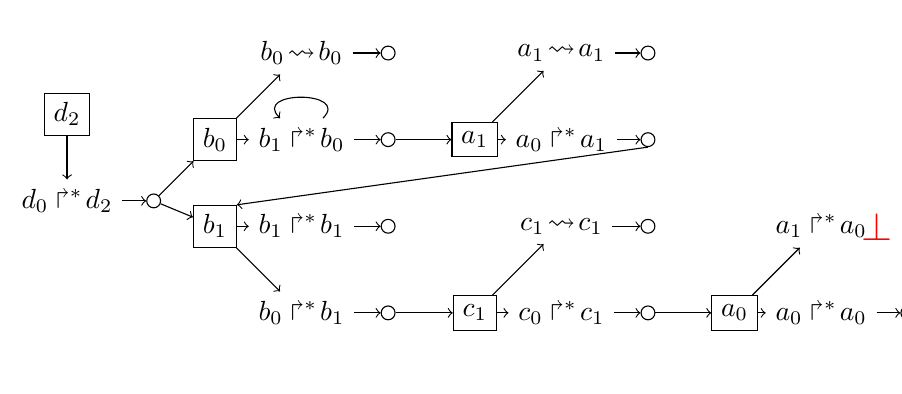
\begin{tikzpicture}[aS,node distance=1.1cm,shorthandon]
\path[use as bounding box] (-0.5,-2.1) rectangle (10.25,2.2);

\node[Aobj] (d02) {$\PHobjectif{d_0}{d_2}$};
\node[Aproc,above of=d02] (d2) {$d_2$};

\node[Asol,right of=d02] (d02s2) {};
\node[Aproc,above right of=d02s2] (b0) {$b_0$};
\node[Aobj,right of=b0] (b10) {$\PHobjectif{b_1}{b_0}$};
\node[Asol,right of=b10] (b10s) {};
\node[Aproc,right of=b10s] (a1) {$a_1$};
\node[Aobj,right of=a1] (a01) {$\PHobjectif{a_0}{a_1}$};
\node[Asol,right of=a01] (a01s) {};

\node[Aproc, below of=b0] (b1) {$b_1$};
\node[Aobj,right of=b1] (b11) {$\PHobjectif{b_1}{b_1}$};
\node[Asol,right of=b11] (b11s) {};
\node[Aobj,below of=b11] (b01) {$\PHobjectif{b_0}{b_1}$};
\node[Asol,right of=b01] (b01s) {};
\node[Aproc,right of=b01s] (c1) {$c_1$};
\node[Aobj,right of=c1] (c01) {$\PHobjectif{c_0}{c_1}$};
\node[Asol,right of=c01] (c01s) {};
\node[Aproc,right of=c01s] (a0) {$a_0$};
\node[Aobj,right of=a0] (a00) {$\PHobjectif{a_0}{a_0}$};
\node[Asol,right of=a00] (a00s) {};

\node[Aobj,above of=b10] (b00) {$\obj{b_0}{b_0}$};
\node[Asol,right of=b00] (b00s) {};
\node[Aobj,above of=a01] (a11) {$\obj{a_1}{a_1}$};
\node[Asol,right of=a11] (a11s) {};
\node[Aobj,above of=c01] (c11) {$\obj{c_1}{c_1}$};
\node[Asol,right of=c11] (c11s) {};
\node[Aobj,above of=a00] (a10) {$\PHobjectif{a_1}{a_0}$};
\node at (a10.east) {\Large\color{red}\textbf{$\bot$}};

\path
  (b10) edge[loop,min distance=5mm] (b10)
 ;
\path
(d02) edge (d02s2) (d02s2) edge (b1) edge (b0)
(a01) edge (a01s) (a01s.south) edge (b1.north east)
(b10) edge (b10s) (b10s) edge (a1)
(b11) edge (b11s)
(a1) edge (a01)
(b0) edge (b10) (b1) edge (b11)
(d2) edge (d02)
;
\path
(b00) edge (b00s)
(b0) edge (b00)
 (b1) edge (b01)
 (b01) edge (b01s) (b01s) edge (c1)
 (c1) edge (c01)
 (c01) edge (c01s) (c01s) edge (a0)
 (a0) edge (a00) (a00) edge (a00s)
;
\path
 (c1) edge (c11) (c11) edge (c11s)
(a0) edge (a10)
(a1) edge (a11)
(a11) edge (a11s)
;

%\node[right of=a01s] {\textbf{\Large\color{darkyellow}Inconc}};

\end{tikzpicture}%
}

% Structure abstraite / Sur-approximation / Non
\def \saono {%
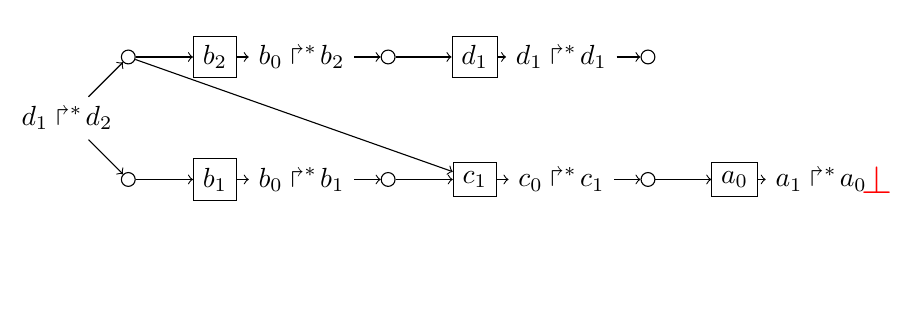
\begin{tikzpicture}[aS,node distance=1.1cm,shorthandon]
\path[use as bounding box] (-0.5,-2.1) rectangle (10.25,1.15);

\node[Aobj] (d12) {$\PHobjectif{d_1}{d_2}$};
\node[Asol,above right of=d12] (d12s1) {};
\node[Aproc, right of=d12s1] (b2) {$b_2$};
\node[Aobj,right of=b2] (b02) {$\PHobjectif{b_0}{b_2}$};
\node[Asol,right of=b02] (b02s) {};
\node[Aproc,right of=b02s] (d1) {$d_1$};
\node[Aobj,right of=d1] (d11) {$\PHobjectif{d_1}{d_1}$};
\node[Asol,right of=d11] (d11s) {};

\node[Asol,below right of=d12] (d12s2) {};
\node[Aproc, right of=d12s2] (b1) {$b_1$};
\node[Aobj,right of=b1] (b01) {$\PHobjectif{b_0}{b_1}$};
\node[Asol,right of=b01] (b01s) {};
\node[Aproc,right of=b01s] (c1) {$c_1$};
\node[Aobj,right of=c1] (c01) {$\PHobjectif{c_0}{c_1}$};
\node[Asol,right of=c01] (c01s) {};
\node[Aproc,right of=c01s] (a0) {$a_0$};
\node[Aobj,right of=a0] (a10) {$\PHobjectif{a_1}{a_0}$};
\node at (a10.east) {\Large\color{red}\textbf{$\bot$}};

\path
(d12) edge (d12s1) edge (d12s2) (d12s1) edge (b2) edge (c1) (d12s2) edge (b1)
(b01) edge (b01s) (b01s) edge (c1)
(b02) edge (b02s) (b02s) edge (d1)
(c01) edge (c01s) (c01s) edge (a0)
(d11) edge (d11s)
(a0) edge (a10)
(b1) edge (b01)
(b2) edge (b02)
(c1) edge (c01)
(d1) edge (d11)
;
%\only<\value{anim1}>{ \node[above right of=c01s] {\textbf{\Large\color{red}No}};}
\end{tikzpicture}%
}

% Structure abstraite / Sur-approximation / Inconclusif
\def \saoinconc {%
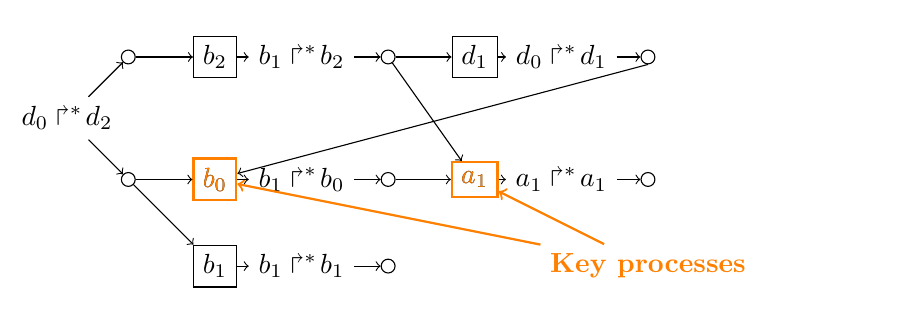
\begin{tikzpicture}[aS,node distance=1.1cm,shorthandon]
\path[use as bounding box] (-0.5,-2.1) rectangle (10.25,1.15);

\node[Aobj] (d02) {$\PHobjectif{d_0}{d_2}$};
\node[Asol,above right of=d02] (d02s1) {};

\node[Aproc, right of=d02s1] (b2) {$b_2$};
\node[Aobj,right of=b2] (b12) {$\PHobjectif{b_1}{b_2}$};
\node[Asol,right of=b12] (b12s) {};
\node[Aproc,right of=b12s] (d1) {$d_1$};
\node[Aobj,right of=d1] (d01) {$\PHobjectif{d_0}{d_1}$};
\node[Asol,right of=d01] (d01s) {};

\node[Asol,below right of=d02] (d02s2) {};
%<-3>
\node<-\tof>[Aproc, right of=d02s2] (b0) {$b_0$};
\node<\tokp>[orange, thick, Aproc, right of=d02s2] (b0) {$b_0$};
\node[Aobj,right of=b0] (b10) {$\PHobjectif{b_1}{b_0}$};
\node[Asol,right of=b10] (b10s) {};
%<-3>
\node<-\tof>[Aproc,right of=b10s] (a1) {$a_1$};
\node<\tokp>[orange, thick, Aproc,right of=b10s] (a1) {$a_1$};
\node[Aobj,right of=a1] (a11) {$\PHobjectif{a_1}{a_1}$};
\node[Asol,right of=a11] (a11s) {};

\node[Aproc, below of=b0] (b1) {$b_1$};
\node[Aobj,right of=b1] (b11) {$\PHobjectif{b_1}{b_1}$};
\node[Asol,right of=b11] (b11s) {};

\node<\tokp>[orange, font=\bfseries,below of=a11s] (kp) {Key processes};
\path<\tokp>[orange, thick]
        (kp) edge (a1)
        (kp) edge (b0)
;
\path
(d02) edge (d02s1) edge (d02s2) (d02s1) edge (b2) (d02s2) edge (b1) edge (b0)
(a11) edge (a11s)
(b10) edge (b10s) (b10s) edge (a1)
(b11) edge (b11s)
(b12) edge (b12s) (b12s) edge (d1) edge (a1)
(d01) edge (d01s) (d01s.south) edge (b0)
(a1) edge (a11)
(b0) edge (b10) (b1) edge (b11) (b2) edge (b12)
(d1) edge (d01)
;
%\node[below right of=d01s] {\textbf{\Large\color{yellow}Inconc}};
\end{tikzpicture}%
}


\def \sasaquant {

    \begin{tikzpicture}[aS,node distance=1.1cm,shorthandon]
    
    % \path[use as bounding box] (-0.5,-3.1) rectangle (10.25,1.15);
     \path[use as bounding box] (3,0) rectangle (10.25,-2.15);

      \node[Aproc] (d2) {$d_2$};
      \node[Aobj,below of=d2] (d12) {$\PHobjectif{d_1}{d_2}{\color{blue}(0.14)}$};
      \node[Asol,right of=d12] (d12s) {};
      

      \node[Aproc,right of=d12s] (bbs) {$b_1,bs_1,\rlab{e_1}$};
      \node[Asol,right of=bbs] (bbss) {};

      \node[Aproc,right  of=bbss] (b1) {$b_1$};
      \node[Aobj,right of=b1] (b01) {$\PHobjectif{b_0}{b_1}{\color{blue}(0.05)}$};
      \node[Asol,right of=b01] (b01s) {};
      %\node[Aobj,below left of=a1] (a01) {$\PHobj{a_0}{a_1}$};
      %\node[Asol,below of=a01] (a01s) {};
      \node[Aproc,right of=b01s] (a1) {$\rlab{c_1},a_1$};
      \node[Aobj,right of=a1] (a11) {$\PHobjectif{a_1}{a_1}{\color{blue}(1)}$};
      \node[Asol,right of=a11] (a11s) {};
      \node[RAobj,above right of=a1] (c11) {$\PHobjectif{c_1}{c_1}{\color{blue}(1)}$};
      \node[RAsol,right of=c11] (c11s) {{\Large\color{red}\textbf{$\otimes$}}};
      %\node[Aobj,below left of=b0] (b10) {$\PHobj{b_1}{b_0}$};
      %\node[Asol,below of=b10] (b10s) {};

      \node[Aproc,below right  of=bbss] (bs1) {$bs_1$};
      \node[Aobj,right of=bs1] (bs01) {$\PHobjectif{bs_0}{bs_1}{\color{blue}(1)}$};
      \node[Asol,right of=bs01] (bs01s) {};
      %\node[Aobj,below right of=b1] (b01) {$\PHobj{b_0}{b_1}$};
      %\node[Asol,below of=b01] (b01s) {};
      \node[Aproc,right of=bs01s] (as1) {$a_1$};
      \node[Aobj,right of=as1] (as11) {$\PHobjectif{a_1}{a_1}{\color{blue}(1)}$};
      \node[Asol,right of=as11] (as11s) {};
      %\node[Aobj,below right of=a0] (a10) {$\PHobj{a_1}{a_0}$};
      %\node[Asol,below of=a10] (a10s) {};

      \node[RAproc,above right of=bbss] (e1) {$e_1$};
      \node[RAobj,right of=e1] (e01) {$\PHobjectif{e_0}{e_1}{\color{blue}(1)}$};
      \node[RAsol,right of=e01] (e01s) {{\Large\color{red}\textbf{$\otimes$}}};

      \path
      (d2) edge (d12)
      (d12) edge (d12s)
      (d12s) edge (bbs)
      (bbs) edge (bbss)
      (bbss) edge (bs1) edge (b1) edge[red] (e1)

      (b1) edge (b01) 
      (b01) edge (b01s)
      (b01s) edge (a1)
      (a1) edge (a11)
      (a11) edge (a11s)
      (a1) edge[red] (c11)
      (c11) edge[red] (c11s)
      %(a0) edge (a10) edge (a00)
      %(a10) edge (a10s)
      %(a00) edge (a00s)

      (bs1) edge (bs01) 
      (bs01) edge (bs01s)
      (bs01s) edge (as1)
      (as1) edge (as11)
      (as11) edge (as11s) 
      %(b01) edge (b01s)
      %(b01s) edge (a0)
      %(b11) edge (b11s)

      (e1) edge[red] (e01) 
      (e01) edge[red] (e01s)
      ;
      \end{tikzpicture}


}

%%% Exemple pour la définition des an %%%
\def \exandef {
\path[use as bounding box] (-0.5,-0.5) rectangle (6.5,4.5);

\TSort{(0,1)}{a}{3}{l}
\TSort{(3,1)}{b}{2}{l}
\TSort{(6,1)}{c}{3}{l}

\path[local transitions]
  (a_0) edge node[auto] {$b_0$} (a_1)
  (a_1) edge (a_0)
  (a_0) edge[bend right=60] node[right] {$b_0,c_0$} (a_2)
  (c_0) edge node[auto] {$a_1$} (c_1)
  (c_1) edge node[auto] {$b_0$} (c_2)
  (c_1) edge node[auto] {$b_1$} (c_0)
  (b_0) edge (b_1)
  (b_1) edge node[auto] {$a_0$} (b_0)
;
}

%%% Exemple pour la définition des an %%%
\def \exanaspdef {
\path[use as bounding box] (-0.5,-0.5) rectangle (6.5,4.5);

\TSort{(3,1.5)}{a}{3}{l}

\path[local transitions]
  (a_0) edge node[auto] {$b_0$} (a_1)
  (a_1) edge (a_0)
  (a_0) edge[bend right=60] node[right] {$b_0,c_0$} (a_2)
;
}






%%% Citations
\newcommand{\citeegfra}{\quad\tval{\ex{egfr20}}: \tcite{Epidermal Growth Factor Receptor, by Özgür Sahin \textit{et al.}}}
\newcommand{\citeegfrb}{\quad\tval{\ex{egfr104}}: \tcite{Epidermal Growth Factor Receptor, by Regina Samaga \textit{et al.}}}
\newcommand{\citetcrsiga}{\quad\tval{\ex{tcrsig40}}: \tcite{T-Cell Receptor Signaling, by Steffen Klamt \textit{et al.}}}
\newcommand{\citetcrsigb}{\quad\tval{\ex{tcrsig94}}: \tcite{T-Cell Receptor Signaling, by Julio Saez-Rodriguez \textit{et al.}}}

\newcommand{\citemodels}{\bigskip\citeegfra\\\citeegfrb\\\citetcrsiga\\\citetcrsigb}

\newcommand{\citepmrtcsb}{Paulevé, Magnin, Roux in \textit{Transactions on Computational Systems Biology}, 2011}
\newcommand{\citepmrmscs}{Paulevé, Magnin, Roux in \textit{Mathematical Structures in Computer Science}, 2012}
\newcommand{\citefpimrcmsb}{{\small Folschette, Paulevé, Inoue, Magnin, Roux\\in \textit{Computational Methods in Systems Biology}, 2012}}
%\newcommand{\crcbmfma}{Richard, Comet, Bernot in Modern Formal Methods and App., 2006}
\newcommand{\citedejong}{De Jong in \textit{Journal of Computational Biology}, 2002}
\newcommand{\citerichardcomet}{Richard, Comet in \textit{Discrete Applied Mathematics}, 2007}
\newcommand{\citeremy}{Remy, Ruet, Thieffry in \textit{Advances in Applied Mathematics}, 2008}
\newcommand{\citesmbionet}{Bernot, Comet, Richard, Guespin in \textit{Journal of Theoretical Biology}, 2004}
\newcommand{\citeito}{Ito, Izumi, Hagihara, Yonezaki in \textit{BioInformatics and BioEngineering}, 2010}
\newcommand{\citeatfb}{Abou-Jaoudé et al, in \textit{Frontiers in Bioengineering and Biotechnology}, 2015}
\newcommand{\citelui}{Liu et al, in \textit{Journal of Bioinformatics and Computational Biology}, 2012}


%%%%%%%%     introduction
\section{Introduction}
% Diapo d'intro
\begin{frame}[c]
  \frametitle{Context}
%rajouter le titre (version courte) dans toute les slides
\begin{center}
  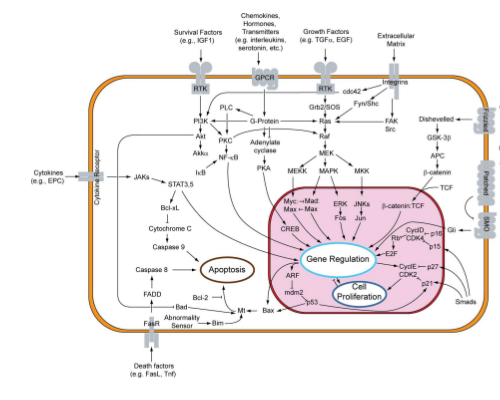
\includegraphics[scale=0.55]{images/cellule_description_lui.png}
\end{center}
\begin{center}
{\tiny \color{darkgreen}[\citelui]}
\end{center}

%\tcite{Wikipédia}

\begin{itemize}
\item Cellular processes are driven by networks of biological interactions.
\item Formal modelling and analysis of Biological Regulatory Network.
\item Static analysis of properties.
\end{itemize}

%Cellular processes are driven by networks of biological reactions. Cells rely on the tight coordination of these pathways to achieve proper functioning.
%With the help of signaling pathway, a cell senses changes in its environnement or internal state. This information is then passed on via cascades of biochemical 
%reactions to the appropriate mechanisms which respond by modifying the metabolic and transcriptiona activities. this in turn modifies the behavior of the cell.

%Consequently, the dynamics of biopathways play a crucial role in determinig cellular functions.

%Examples: circadian rhythm, the apoptosis pathway inducing programmed cell death, cell differentiation.

%\textcolor{couleurtheme}{$\Rightarrow$} \fbox{\tval{\large The need of comprehension of biological systems}} \textcolor{couleurtheme}{$\Leftarrow$}


%\textcolor{couleurtheme}{$\Rightarrow$} \fbox{\tval{\large Allow efficient translation from Process Hitting to BRN}} \textcolor{couleurtheme}{$\Leftarrow$}

\end{frame}

\begin{frame}[c]
  \frametitle{Motivation}
 \framesubtitle{stem cell differentiation}

\begin{center}
  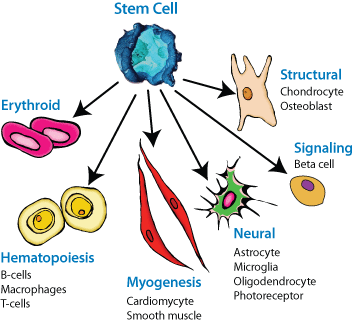
\includegraphics[scale=0.42]{images/illustration_differentiation.png}
  % \multiinclude[format=gif, scale=0.5]{images/illustration_differentiation.gif}
\end{center}
\begin{center}
{\tiny \color{darkgreen} [https://www.systembio.com/stem-cell-research/differentiation-reporters/overview]}
\end{center}
%\tcite{system Biosciences}

\begin{itemize}
\item Loss of  capability \tval{differentiation}  %expliquer la notion de perte de capacité sur la figure.
\item Which transitions (operations) are responsible of \tval{Bifurcations} ? 
\item From which state ?
\end{itemize}
\end{frame}

\begin{frame}[c]
  \frametitle{Contribution}
%system dynamique
%Bifurcations
%rajouter une autre image pour illustrer pour qu'on voit que c'est toujours des états qui changes
\begin{center}
  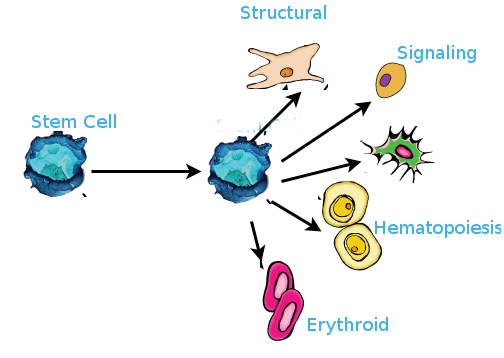
\includegraphics[scale=0.3]{images/illustration_differentiation_newio1.png}
  % \multiinclude[format=gif, scale=0.5]{images/illustration_differentiation.gif}
\end{center}


\begin{itemize}
\item Bifurcation transitions can be  expressed in temporal logic formula
\item {\bf "Relaxation"} :\\ verification of CTL formula (\tval{PSPACE (complete)})\\
       $\Rightarrow$ NP problem which can be easily expressed in SAT/ASP %trouver l'orthagraphe de easely
\item {\bf Contribution} : $$
\left\{
    \begin{array}{lcl}
        \mbox{AI (Artificial inteligence)} &\\  %rajouter un signe entre les deux
        \mbox{+} & $\Longrightarrow$ \mbox{\tval{formal approximation of bifurcations}} \\
        \mbox{AI (Abstract interpretation)} &
    \end{array}
\right.
$$ 
\end{itemize}
\end{frame}


%\tableofcontents

\section{Automata Network}
% Définition du Process Hitting + sortes coopératives

%mettre un RRB ----> en AAN  ----> STate graph 
%rajouter une slide
\begin{frame}
\frametitle{Biological networks modelling}
\begin{tikzpicture}
\node (brn) at (0,5) {\begin{tikzpicture}[auto,scale=0.9] 
                                                 \path[use as bounding box] (-0.7,-0.3) rectangle (2.5,2);

                                                              \node[qgre,scale=0.8] (a) at (0,2) {a};
                                                              \node[mod,scale=0.8] (i) at (1,1) {i};
                                                              \node[qgre,scale=0.8] (b) at (0,0) {b};
                                                              \node[qgre,scale=0.8] (c) at (2,1) {c};
                                                              \path
                                                                (a) edge[inhN,scale=0.1] (i)
                                                                (b) edge[actN,scale=0.1] (i)
                                                                (i) edge[st,scale=0.1]  (c);
                                                              
                                                 \end{tikzpicture}};
\node[scale=0.6] (an) at (7,5) {\begin{tikzpicture}
\exandef
\end{tikzpicture}};
\node[scale=0.6] (sg) at (2,1) {
\begin{tikzpicture}[]},line join=bevel,font=\LARGE]
%%
  \node (6) at (405.0bp,18.0bp) [reach,nd4] {$\langle a_2,b_1,c_0\rangle$};
  \node (2) at (405.0bp,90.0bp) [reach,nd3] {$\langle a_2,b_0,c_0\rangle$};
  \node (1) at (570.0bp,90.0bp) [reach,nd1] {$\langle a_1,b_0,c_0\rangle$};
  \node (0) at (469.0bp,162.0bp) [reach,nd0] {$s_0 = \langle a_0,b_0,c_0\rangle$};
  \node (4) at (469.0bp,234.0bp) [reach,nd5] {$\langle a_0,b_1,c_0\rangle$};
 
 
  \draw [->,arc3] (0) ..controls (445.65bp,135.46bp) and (435.95bp,124.86bp)  .. (2);
  \draw [->,arc5] (0) ..controls (475.71bp,188.03bp) and (475.94bp,197.36bp)  .. (4);
  \draw [->,arc4] (2) ..controls (405.0bp,63.983bp) and (405.0bp,54.712bp)  .. (6);
  \draw [->,arc1] (0) ..controls (499.93bp,134.79bp) and (517.41bp,122.58bp)  .. (1);
  \draw [->,arc2] (1) ..controls (539.0bp,117.26bp) and (521.52bp,129.47bp)  .. (0);
  \draw [->,arc5] (4) ..controls (462.3bp,208.35bp) and (462.06bp,199.03bp)  .. (0);
 
%
\end{tikzpicture}

};
\path 
(brn) edge[->,line width=8pt, color=lightgray] (an)
(an) edge[->,line width=8pt, color=lightgray,bend left] (sg)
;

\end{tikzpicture}
\end{frame}


\begin{frame}
  \frametitle{Automata Networks}
  %\framesubtitle{\tcite{Paulev\'e et al. 2012}}


\begin{columns}
\begin{column}{0.6\textwidth}
% 1 : Sortes
\only<1>{
\tikzstyle{process}=[circle,minimum size=15pt,font=\footnotesize,inner sep=1pt]
\tikzstyle{tick label}=[color=white, font=\footnotesize]
\tikzstyle{tick}=[transparent]
\tikzstyle{hit}=[transparent]
\tikzstyle{selfhit}=[transparent, min distance=30pt,curve to]
\tikzstyle{bounce}=[transparent]
\tikzstyle{hlhit}=[transparent]
\tikzstyle{local transitions}=[transparent]
\begin{center}\scalebox{\scaleex}{
\begin{tikzpicture}
\exandef
\end{tikzpicture}
}\end{center}
}

% 2 : Processus
\only<2>{
\tikzstyle{process}=[circle,draw,minimum size=15pt,font=\footnotesize,inner sep=1pt]
\tikzstyle{tick label}=[font=\footnotesize]
\tikzstyle{tick}=[densely dotted]
\tikzstyle{hit}=[transparent]
\tikzstyle{selfhit}=[transparent, min distance=30pt,curve to]
\tikzstyle{bounce}=[transparent]
\tikzstyle{hlhit}=[transparent]
\tikzstyle{local transitions}=[transparent]
\begin{center}\scalebox{\scaleex}{
\begin{tikzpicture}
\exandef
\end{tikzpicture}
}\end{center}
}

% 3 : États
\only<3>{
\tikzstyle{hit}=[transparent]
\tikzstyle{selfhit}=[transparent, min distance=30pt,curve to]
\tikzstyle{bounce}=[transparent]
\tikzstyle{hlhit}=[transparent]
\tikzstyle{local transitions}=[transparent]
\begin{center}\scalebox{\scaleex}{
\begin{tikzpicture}
\exandef

\TState{3}{a_0,b_0,c_0}
\end{tikzpicture}
}\end{center}
}

% 4 : Actions
\only<4->{
\tikzstyle{tick}=[densely dotted]
\tikzstyle{hit}=[->,>=angle 45]
\tikzstyle{selfhit}=[min distance=30pt,curve to]
\tikzstyle{bounce}=[densely dotted,>=stealth',->]
\tikzstyle{hlhit}=[very thick]
\begin{center}\scalebox{\scaleex}{
\begin{tikzpicture}
\exandef
\TState{4}{a_0,b_0,c_0}
\TState{5}{a_1,b_0,c_0}
\TState{6}{a_0,b_0,c_0}
\TState{7}{a_2,b_0,c_0}
\TState{8}{a_2,b_1,c_0}
\end{tikzpicture}
}\end{center}
}
\end{column}

\begin{column}{0.4\textwidth}
\begin{figure}[p]
\centering

\scalebox{0.4}{
\only<4>{
\tikzstyle{arc0}=[transparent]
\tikzstyle{nd0}=[]
\tikzstyle{arc1}=[transparent]
\tikzstyle{nd1}=[transparent]
\tikzstyle{arc2}=[transparent]
\tikzstyle{nd2}=[transparent]
\tikzstyle{arc3}=[transparent]
\tikzstyle{nd3}=[transparent]
\tikzstyle{arc4}=[transparent]
\tikzstyle{nd4}=[transparent]
\tikzstyle{arc5}=[transparent]
\tikzstyle{nd5}=[transparent]

\begin{tikzpicture}[]},line join=bevel,font=\LARGE]
%%
  \node (6) at (405.0bp,18.0bp) [reach,nd4] {$\langle a_2,b_1,c_0\rangle$};
  \node (2) at (405.0bp,90.0bp) [reach,nd3] {$\langle a_2,b_0,c_0\rangle$};
  \node (1) at (570.0bp,90.0bp) [reach,nd1] {$\langle a_1,b_0,c_0\rangle$};
  \node (0) at (469.0bp,162.0bp) [reach,nd0] {$s_0 = \langle a_0,b_0,c_0\rangle$};
  \node (4) at (469.0bp,234.0bp) [reach,nd5] {$\langle a_0,b_1,c_0\rangle$};
 
 
  \draw [->,arc3] (0) ..controls (445.65bp,135.46bp) and (435.95bp,124.86bp)  .. (2);
  \draw [->,arc5] (0) ..controls (475.71bp,188.03bp) and (475.94bp,197.36bp)  .. (4);
  \draw [->,arc4] (2) ..controls (405.0bp,63.983bp) and (405.0bp,54.712bp)  .. (6);
  \draw [->,arc1] (0) ..controls (499.93bp,134.79bp) and (517.41bp,122.58bp)  .. (1);
  \draw [->,arc2] (1) ..controls (539.0bp,117.26bp) and (521.52bp,129.47bp)  .. (0);
  \draw [->,arc5] (4) ..controls (462.3bp,208.35bp) and (462.06bp,199.03bp)  .. (0);
 
%
\end{tikzpicture}


}
\only<5>{
\tikzstyle{arc0}=[->]
\tikzstyle{nd0}=[]
\tikzstyle{arc1}=[->]
\tikzstyle{nd1}=[]
\tikzstyle{arc2}=[transparent]
\tikzstyle{nd2}=[transparent]
\tikzstyle{arc3}=[transparent]
\tikzstyle{nd3}=[transparent]
\tikzstyle{arc4}=[transparent]
\tikzstyle{nd4}=[transparent]
\tikzstyle{arc5}=[transparent]
\tikzstyle{nd5}=[transparent]

\begin{tikzpicture}[]},line join=bevel,font=\LARGE]
%%
  \node (6) at (405.0bp,18.0bp) [reach,nd4] {$\langle a_2,b_1,c_0\rangle$};
  \node (2) at (405.0bp,90.0bp) [reach,nd3] {$\langle a_2,b_0,c_0\rangle$};
  \node (1) at (570.0bp,90.0bp) [reach,nd1] {$\langle a_1,b_0,c_0\rangle$};
  \node (0) at (469.0bp,162.0bp) [reach,nd0] {$s_0 = \langle a_0,b_0,c_0\rangle$};
  \node (4) at (469.0bp,234.0bp) [reach,nd5] {$\langle a_0,b_1,c_0\rangle$};
 
 
  \draw [->,arc3] (0) ..controls (445.65bp,135.46bp) and (435.95bp,124.86bp)  .. (2);
  \draw [->,arc5] (0) ..controls (475.71bp,188.03bp) and (475.94bp,197.36bp)  .. (4);
  \draw [->,arc4] (2) ..controls (405.0bp,63.983bp) and (405.0bp,54.712bp)  .. (6);
  \draw [->,arc1] (0) ..controls (499.93bp,134.79bp) and (517.41bp,122.58bp)  .. (1);
  \draw [->,arc2] (1) ..controls (539.0bp,117.26bp) and (521.52bp,129.47bp)  .. (0);
  \draw [->,arc5] (4) ..controls (462.3bp,208.35bp) and (462.06bp,199.03bp)  .. (0);
 
%
\end{tikzpicture}


}
\only<6>{
\tikzstyle{arc0}=[->]
\tikzstyle{nd0}=[]
\tikzstyle{arc1}=[->]
\tikzstyle{nd1}=[]
\tikzstyle{arc2}=[->]
\tikzstyle{nd2}=[]
\tikzstyle{arc3}=[transparent]
\tikzstyle{nd3}=[transparent]
\tikzstyle{arc4}=[transparent]
\tikzstyle{nd4}=[transparent]
\tikzstyle{arc5}=[transparent]
\tikzstyle{nd5}=[transparent]

\begin{tikzpicture}[]},line join=bevel,font=\LARGE]
%%
  \node (6) at (405.0bp,18.0bp) [reach,nd4] {$\langle a_2,b_1,c_0\rangle$};
  \node (2) at (405.0bp,90.0bp) [reach,nd3] {$\langle a_2,b_0,c_0\rangle$};
  \node (1) at (570.0bp,90.0bp) [reach,nd1] {$\langle a_1,b_0,c_0\rangle$};
  \node (0) at (469.0bp,162.0bp) [reach,nd0] {$s_0 = \langle a_0,b_0,c_0\rangle$};
  \node (4) at (469.0bp,234.0bp) [reach,nd5] {$\langle a_0,b_1,c_0\rangle$};
 
 
  \draw [->,arc3] (0) ..controls (445.65bp,135.46bp) and (435.95bp,124.86bp)  .. (2);
  \draw [->,arc5] (0) ..controls (475.71bp,188.03bp) and (475.94bp,197.36bp)  .. (4);
  \draw [->,arc4] (2) ..controls (405.0bp,63.983bp) and (405.0bp,54.712bp)  .. (6);
  \draw [->,arc1] (0) ..controls (499.93bp,134.79bp) and (517.41bp,122.58bp)  .. (1);
  \draw [->,arc2] (1) ..controls (539.0bp,117.26bp) and (521.52bp,129.47bp)  .. (0);
  \draw [->,arc5] (4) ..controls (462.3bp,208.35bp) and (462.06bp,199.03bp)  .. (0);
 
%
\end{tikzpicture}


}
\only<7>{
\tikzstyle{arc0}=[->]
\tikzstyle{nd0}=[]
\tikzstyle{arc1}=[->]
\tikzstyle{nd1}=[]
\tikzstyle{arc2}=[->]
\tikzstyle{nd2}=[]
\tikzstyle{arc3}=[->]
\tikzstyle{nd3}=[]
\tikzstyle{arc4}=[transparent]
\tikzstyle{nd4}=[transparent]
\tikzstyle{arc5}=[transparent]
\tikzstyle{nd5}=[transparent]

\begin{tikzpicture}[]},line join=bevel,font=\LARGE]
%%
  \node (6) at (405.0bp,18.0bp) [reach,nd4] {$\langle a_2,b_1,c_0\rangle$};
  \node (2) at (405.0bp,90.0bp) [reach,nd3] {$\langle a_2,b_0,c_0\rangle$};
  \node (1) at (570.0bp,90.0bp) [reach,nd1] {$\langle a_1,b_0,c_0\rangle$};
  \node (0) at (469.0bp,162.0bp) [reach,nd0] {$s_0 = \langle a_0,b_0,c_0\rangle$};
  \node (4) at (469.0bp,234.0bp) [reach,nd5] {$\langle a_0,b_1,c_0\rangle$};
 
 
  \draw [->,arc3] (0) ..controls (445.65bp,135.46bp) and (435.95bp,124.86bp)  .. (2);
  \draw [->,arc5] (0) ..controls (475.71bp,188.03bp) and (475.94bp,197.36bp)  .. (4);
  \draw [->,arc4] (2) ..controls (405.0bp,63.983bp) and (405.0bp,54.712bp)  .. (6);
  \draw [->,arc1] (0) ..controls (499.93bp,134.79bp) and (517.41bp,122.58bp)  .. (1);
  \draw [->,arc2] (1) ..controls (539.0bp,117.26bp) and (521.52bp,129.47bp)  .. (0);
  \draw [->,arc5] (4) ..controls (462.3bp,208.35bp) and (462.06bp,199.03bp)  .. (0);
 
%
\end{tikzpicture}


}
\only<8>{
\tikzstyle{arc0}=[->]
\tikzstyle{nd0}=[]
\tikzstyle{arc1}=[->]
\tikzstyle{nd1}=[]
\tikzstyle{arc2}=[->]
\tikzstyle{nd2}=[]
\tikzstyle{arc3}=[->]
\tikzstyle{nd3}=[]
\tikzstyle{arc4}=[->]
\tikzstyle{nd4}=[]
\tikzstyle{arc5}=[transparent]
\tikzstyle{nd5}=[transparent]

\begin{tikzpicture}[]},line join=bevel,font=\LARGE]
%%
  \node (6) at (405.0bp,18.0bp) [reach,nd4] {$\langle a_2,b_1,c_0\rangle$};
  \node (2) at (405.0bp,90.0bp) [reach,nd3] {$\langle a_2,b_0,c_0\rangle$};
  \node (1) at (570.0bp,90.0bp) [reach,nd1] {$\langle a_1,b_0,c_0\rangle$};
  \node (0) at (469.0bp,162.0bp) [reach,nd0] {$s_0 = \langle a_0,b_0,c_0\rangle$};
  \node (4) at (469.0bp,234.0bp) [reach,nd5] {$\langle a_0,b_1,c_0\rangle$};
 
 
  \draw [->,arc3] (0) ..controls (445.65bp,135.46bp) and (435.95bp,124.86bp)  .. (2);
  \draw [->,arc5] (0) ..controls (475.71bp,188.03bp) and (475.94bp,197.36bp)  .. (4);
  \draw [->,arc4] (2) ..controls (405.0bp,63.983bp) and (405.0bp,54.712bp)  .. (6);
  \draw [->,arc1] (0) ..controls (499.93bp,134.79bp) and (517.41bp,122.58bp)  .. (1);
  \draw [->,arc2] (1) ..controls (539.0bp,117.26bp) and (521.52bp,129.47bp)  .. (0);
  \draw [->,arc5] (4) ..controls (462.3bp,208.35bp) and (462.06bp,199.03bp)  .. (0);
 
%
\end{tikzpicture}


}
\only<9>{
\tikzstyle{arc0}=[->]
\tikzstyle{nd0}=[]
\tikzstyle{arc1}=[->]
\tikzstyle{nd1}=[]
\tikzstyle{arc2}=[->]
\tikzstyle{nd2}=[]
\tikzstyle{arc3}=[->]
\tikzstyle{nd3}=[]
\tikzstyle{arc4}=[->]
\tikzstyle{nd4}=[]
\tikzstyle{arc5}=[->]
\tikzstyle{nd5}=[]

\begin{tikzpicture}[]},line join=bevel,font=\LARGE]
%%
  \node (6) at (405.0bp,18.0bp) [reach,nd4] {$\langle a_2,b_1,c_0\rangle$};
  \node (2) at (405.0bp,90.0bp) [reach,nd3] {$\langle a_2,b_0,c_0\rangle$};
  \node (1) at (570.0bp,90.0bp) [reach,nd1] {$\langle a_1,b_0,c_0\rangle$};
  \node (0) at (469.0bp,162.0bp) [reach,nd0] {$s_0 = \langle a_0,b_0,c_0\rangle$};
  \node (4) at (469.0bp,234.0bp) [reach,nd5] {$\langle a_0,b_1,c_0\rangle$};
 
 
  \draw [->,arc3] (0) ..controls (445.65bp,135.46bp) and (435.95bp,124.86bp)  .. (2);
  \draw [->,arc5] (0) ..controls (475.71bp,188.03bp) and (475.94bp,197.36bp)  .. (4);
  \draw [->,arc4] (2) ..controls (405.0bp,63.983bp) and (405.0bp,54.712bp)  .. (6);
  \draw [->,arc1] (0) ..controls (499.93bp,134.79bp) and (517.41bp,122.58bp)  .. (1);
  \draw [->,arc2] (1) ..controls (539.0bp,117.26bp) and (521.52bp,129.47bp)  .. (0);
  \draw [->,arc5] (4) ..controls (462.3bp,208.35bp) and (462.06bp,199.03bp)  .. (0);
 
%
\end{tikzpicture}


}
}

\end{figure}

\end{column}
\end{columns}
%\medskip

\begin{liste}
  \item \tval{Automata}: components \qex{$a$, $b$, $c$}
\pause[2]
  \item \tval{local states}: levels of expression \qex{$c_0$, $c_1$, $c_2$}
\pause[3]
  \item \tval{States}: sets of active local states%
  \only<3-4>{\qex{$\PHetat{a_0, b_0, c_0}$}}%
  \only<5>{\qex{$\PHetat{a_1, b_0, c_0}$}}%
  \only<6>{\qex{$\PHetat{a_0, b_0, c_0}$}}%
  \only<7>{\qex{$\PHetat{a_2, b_0, c_0}$}}%
  \only<8>{\qex{$\PHetat{a_2, b_1, c_0}$}}
\pause[4]
  \item \tval{Transitions}: dynamics \qex{\only<5>{\underline}{$t_1 = \trans{a_0}{a_1}{b_0}$}, \only<6>{\underline}{$t_2 = \trans{a_1}{a_0}{}$}, \only<7>{\underline}{$t_3 = \trans{a_0}{a_2}{b_0,c_0}$}, \only<8>{\underline}{$t_4 = \trans{b_0}{b_1}{}$}}
\end{liste}
%une seule transition à la fois
%on peut avoir un choix il faut bien expliquer ça.
\end{frame}



%\input{parts/static_analysis.tex}

\section{Static analysis of bifurcations}
\subsection{What is a bifurcation?}
\begin{frame}[c]
 \frametitle{Illustration of bifurcations}
 
%\ref{ex-bifurcations} shows all the possible transitions from $s_0$.
\begin{figure}[p]
\centering

\scalebox{0.4}{

\begin{tikzpicture}[]},line join=bevel,font=\LARGE]
%%
  \node (6) at (405.0bp,18.0bp) [reach] {$\langle \mathbf{\color{blue}a_2},b_1,c_0\rangle$};
  \node (2) at (405.0bp,90.0bp) [reach] {$\langle \mathbf{\color{blue}a_2},b_0,c_0\rangle$};

\node (1) at (570.0bp,90.0bp) [reach] {$\langle a_1,b_0,c_0\rangle$};
  \node (64) at (304.0bp,234.0bp) [reach] {$\langle a_0,b_0,c_1\rangle$};
  \node (0) at (469.0bp,162.0bp) [reach] {$\mathbf{\color{maroon}s_0 = \langle a_0,b_0,c_0\rangle}$};
  \node (5) at (507.0bp,306.0bp) [reach] {$\langle a_1,b_1,c_0\rangle$};
  \node (4) at (469.0bp,234.0bp) [reach] {$\langle a_0,b_1,c_0\rangle$};
  \node (69) at (425.0bp,378.0bp) [reach] {$\langle a_1,b_1,c_1\rangle$};
  \node (68) at (342.0bp,306.0bp) [reach] {$\langle a_0,b_1,c_1\rangle$};
  \node (65) at (232.0bp,450.0bp) [reach] {$\langle a_1,b_0,c_1\rangle$};

  \node[elipse,fill=gray!30] (129) at (88.0bp,90.0bp)  {$\langle a_1,b_0,c_2\rangle$};
  \node[elipse,fill=gray!30] (128) at (139.0bp,162.0bp)  {$\langle a_0,b_0,c_2\rangle$};
  \node[elipse,fill=gray!30] (133) at (112.0bp,306.0bp)  {$\langle a_1,b_1,c_2\rangle$};
  \node[elipse,fill=gray!30] (132) at (139.0bp,234.0bp)  {$\langle a_0,b_1,c_2\rangle$};

  \draw [->] (0) ..controls (445.65bp,135.46bp) and (435.95bp,124.86bp)  .. (2);
  \draw [->] (133) ..controls (121.57bp,280.18bp) and (125.26bp,270.62bp)  .. (132);
  \draw [->,very thick,red] (65) ..controls (104.12bp,424.19bp) and (0.0bp,387.99bp)  ..  (0.0bp,307.0bp) .. controls (0.0bp,307.0bp) and (0.0bp,307.0bp)  ..  node[auto,font=\huge,fill=white]{$t_8$} (0.0bp,233.0bp) .. controls (0.0bp,185.75bp) and (35.64bp,141.13bp)  .. (129);
  \draw [->] (65) ..controls (223.97bp,401.24bp) and (228.52bp,336.68bp)  .. (251.0bp,288.0bp) .. controls (255.96bp,277.25bp) and (263.67bp,266.89bp)  .. (64);
  \draw [->] (5) ..controls (483.32bp,333.07bp) and (470.02bp,344.55bp)  .. (69);
  \draw [->,very thick,red] (64) ..controls (244.15bp,207.61bp) and (210.57bp,193.36bp)  .. node[auto,font=\huge,fill=white]{$t_8$} (128);
  \draw [->] (5) ..controls (493.43bp,280.01bp) and (488.11bp,270.2bp)  .. (4);
  \draw [->] (0) ..controls (475.71bp,188.03bp) and (475.94bp,197.36bp)  .. (4);
  \draw [->] (1) ..controls (588.79bp,134.38bp) and (608.0bp,186.55bp)  .. (608.0bp,233.0bp) .. controls (608.0bp,307.0bp) and (608.0bp,307.0bp)  .. (608.0bp,307.0bp) .. controls (608.0bp,366.83bp) and (560.73bp,369.68bp)  .. (507.0bp,396.0bp) .. controls (446.14bp,425.81bp) and (370.03bp,438.87bp)  .. (65);
  \draw [->] (1) ..controls (572.33bp,138.66bp) and (571.97bp,203.11bp)  .. (551.0bp,252.0bp) .. controls (546.57bp,262.33bp) and (539.46bp,272.21bp)  .. (5);
  \draw [->] (129) ..controls (68.077bp,117.99bp) and (60.513bp,131.04bp)  .. (57.0bp,144.0bp) .. controls (44.446bp,190.33bp) and (38.221bp,207.83bp)  .. (57.0bp,252.0bp) .. controls (61.945bp,263.63bp) and (70.831bp,273.95bp)  .. (133);
  \draw [->] (128) ..controls (145.71bp,188.03bp) and (145.94bp,197.36bp)  .. (132);
  \draw [->] (69) ..controls (448.8bp,350.83bp) and (462.16bp,339.29bp)  .. (5);
  \draw [->] (2) ..controls (405.0bp,63.983bp) and (405.0bp,54.712bp)  .. (6);
  \draw [->] (0) ..controls (499.93bp,134.79bp) and (517.41bp,122.58bp)  .. (1);
  \draw [->] (68) ..controls (388.56bp,279.34bp) and (412.1bp,266.36bp)  .. (4);
  \draw [->] (68) ..controls (321.75bp,280.09bp) and (316.27bp,270.41bp)  .. (64);
  \draw [->] (1) ..controls (539.0bp,117.26bp) and (521.52bp,129.47bp)  .. (0);
  \draw [->] (65) ..controls (301.71bp,423.72bp) and (343.47bp,408.57bp)  .. (69);
  \draw [->] (64) ..controls (324.32bp,260.04bp) and (329.77bp,269.67bp)  .. (68);
  \draw [->] (69) ..controls (394.58bp,351.34bp) and (381.1bp,339.97bp)  .. (68);
  \draw [->] (128) ..controls (114.09bp,136.08bp) and (106.38bp,125.8bp)  .. (129);
  \draw [->] (64) ..controls (285.73bp,261.68bp) and (275.22bp,274.54bp)  .. (269.0bp,288.0bp) .. controls (248.81bp,331.74bp) and (243.08bp,388.29bp)  .. (65);
  \draw [->] (132) ..controls (132.3bp,208.35bp) and (132.06bp,199.03bp)  .. (128);
  \draw [->] (4) ..controls (462.3bp,208.35bp) and (462.06bp,199.03bp)  .. (0);
  \draw [->] (129) ..controls (113.05bp,116.11bp) and (120.71bp,126.32bp)  .. (128);
%
\end{tikzpicture}


}

%rajouter que quand on a jouer t8 on ne peut plus atteindre a2
%mettre s0 en évidence en gras ou vert 

%\caption{Transition graph of a given AN  from the initial state
%$s_0=\state{a_0,b_0,c_0}$. The goal $a_2$ is in thick/blue; the states connected to the goal are in
%gray; the bifurcations to the goal in thick/red, labelled with the local transitions in the AN definition.}
\label{ex-bifurcations}
\end{figure}

\end{frame}

\begin{frame}
\frametitle{Definition of bifurcation}
\begin{figure}[t]
\centering
\begin{tikzpicture}[node distance=1.5cm]
\node (s0) [circle,fill=gray!60] {$s_0$};
\node (sb) [circle,fill=gray!60,above right of=s0,xshift=2cm] {$s_b$};
\node (g) [circle,fill=blue!20,minimum width=7mm,below right of=sb,xshift=2cm] {$S_{g_1}$};
\node (su) [above right of=sb] {$s_u$};
\node (u) [below right of=su,xshift=5mm] {$\mathbf{\color{red}x}$};
\path[->] (sb) edge[->,red,thick] node[auto] {$t_b$} (su) ;
\path[->,bend left=20,densely dashed]
	(s0) edge (sb)
	(sb) edge (g)
	(s0) edge [bend right=10] (g)
	(su) edge[>={Rays[length=3mm,width=3mm]}] (u)
;
\end{tikzpicture}
\end{figure}

\begin{block}{Definition}
\centering
$t_b$ is a bifurcation transition from $s_0$ to $g_1$

\smallskip
$\Longleftrightarrow$
there exists $s_b$ such that:
%rajouter g1 \in Sg
\begin{align*}
\text{\cI}\enspace &s_u\nreach g_1
&
\text{\cII}\enspace &s_b\reach g_1
&
\text{\cIII}\enspace &s_0\reach s_b
\end{align*}
\end{block}
\end{frame}



\subsection{How to identify bifurcations?}
\begin{frame}[c]
 \frametitle{Formal approximation of reachability}
\framesubtitle{Static analysis by abstract interpretation}
 
The reachability approximations  for ANs introduced in
%\tcite{PMR12-MSCS,FPMR15-TCS}.
{\small \color{darkgreen} [\citepmrmscs] }%revoir les citations


 %\tval{over-approximations} (OA) and \tval{under-approximations} (UA) of the reachability problem:
$$
\begin{align*}
\UA s {s'}&\Rightarrow {\bf s\reach s'} \Rightarrow \OA s {s'}
\end{align*}
$$
\begin{itemize}
\item OA (\tval{over-approximations}): necessary conditions for {\bf $s\reach s'$} %is true only if $\OA s {s'}$ is true
\item UA (\tval{under-approximation}): sufficient conditions for {\bf $s\reach s'$} %is true if  $\UA s {s'}$ is true;
(but the converse does not hold in general)
\end{itemize}

\tval{Interest:}
\begin{itemize}
\item Avoid state space explosion
\item Decide in an efficient way reachability properties
\end{itemize}

\end{frame}


\begin{comment}
\begin{frame}[c]
\frametitle{Formal approximation of reachability}
\framesubtitle{Local Causality Graph}
\begin{columns}
\begin{column}{0.5\textwidth}
\textbf{Idea for OA and UA}
\begin{itemize}
\item Local Causality reasonning
\item \tval{Nodes of LCG}: local states, objectives, solutions. 
\end{itemize}

\textbf {Sufficient condition}:
\begin{itemize}
\item LCG has \tval{no cycle};
\item each objective has \tval{at least one solution};
\item local states of a same pre-condition have no conflicts.
\end{itemize}

\end{column}
\begin{column}{0.5\textwidth}
%presentation of the GLC
  \begin{figure}[h]
 % \scalebox{0.5}{\begin{tikzpicture}[>={Stealth[width=3mm,length=3mm]},line join=bevel,font=\Large]
%%
\node (a_2) at (65.597bp,320.0bp) [draw,rectangle] {$a_2$};
  \node (O_b_0_0) at (28.597bp,61.0bp)  {$\anobj b 0 0$};
  \node (O_c_2_0) at (103.6bp,61.0bp)  {$\anobj c 2 0$};
  \node (c_0) at (102.6bp,133.0bp) [draw,rectangle] {$c_0$};
  \node (O_a_1_2) at (65.597bp,248.0bp)  {$\anobj a 1 2$};
  \node (b_0) at (29.597bp,133.0bp) [draw,rectangle] {$b_0$};
  \node (pintsol1) at (65.597bp,190.5bp) [draw,ellipse] {};
  \node (pintsol2) at (28.597bp,3.5bp) [draw,ellipse] {};
  \draw [->] (O_a_1_2) ..controls (65.597bp,221.59bp) and (65.597bp,212.02bp)  .. (pintsol1);
  \draw [->] (O_b_0_0) ..controls (28.597bp,34.59bp) and (28.597bp,25.018bp)  .. (pintsol2);
  \draw [->] (a_2) ..controls (65.597bp,293.98bp) and (65.597bp,284.71bp)  .. (O_a_1_2);
  \draw [->] (c_0) ..controls (102.95bp,106.98bp) and (103.09bp,97.712bp)  .. (O_c_2_0);
  \draw [->] (pintsol1) ..controls (70.418bp,182.27bp) and (78.07bp,170.79bp)  .. (c_0);
  \draw [->] (b_0) ..controls (29.24bp,106.98bp) and (29.108bp,97.712bp)  .. (O_b_0_0);
  \draw [->] (pintsol1) ..controls (60.907bp,182.27bp) and (53.462bp,170.79bp)  .. (b_0);
%
\end{tikzpicture}
}
  %\hfill
  \scalebox{0.3}{\begin{tikzpicture}[>={Stealth[width=3mm,length=3mm]},line join=bevel,font=\Large]
%%
\node (O_c_1_0) at (103.6bp,248.0bp)  {$\anobj c 1 0$};
  \node (a_2) at (65.597bp,507.0bp) [draw,rectangle] {$a_2$};
  \node (O_b_0_1) at (103.6bp,61.0bp)  {$\anobj b 0 1$};
  \node (O_b_0_0) at (28.597bp,248.0bp)  {$\anobj b 0 0$};
  \node (c_0) at (102.6bp,320.0bp) [draw,rectangle] {$c_0$};
  \node (O_a_1_2) at (65.597bp,435.0bp)  {$\anobj a 1 2$};
  \node (pintsol4) at (103.6bp,190.5bp) [draw,circle] {};
  \node (b_0) at (29.597bp,320.0bp) [draw,rectangle] {$b_0$};
  \node (b_1) at (103.6bp,133.0bp) [draw,rectangle] {$b_1$};
  \node (pintsol1) at (65.597bp,377.5bp) [draw,circle] {};
  \node (pintsol3) at (103.6bp,3.5bp) [draw,circle] {};
  \node (pintsol2) at (28.597bp,190.5bp) [draw,circle] {};
  \draw [->] (b_1) ..controls (103.6bp,106.98bp) and (103.6bp,97.712bp)  .. (O_b_0_1);
  \draw [->] (O_b_0_1) ..controls (103.6bp,34.59bp) and (103.6bp,25.018bp)  .. (pintsol3);
  \draw [->] (O_a_1_2) ..controls (65.597bp,408.59bp) and (65.597bp,399.02bp)  .. (pintsol1);
  \draw [->] (O_b_0_0) ..controls (28.597bp,221.59bp) and (28.597bp,212.02bp)  .. (pintsol2);
  \draw [->] (pintsol4) ..controls (103.6bp,182.05bp) and (103.6bp,171.59bp)  .. (b_1);
  \draw [->] (a_2) ..controls (65.597bp,480.98bp) and (65.597bp,471.71bp)  .. (O_a_1_2);
  \draw [->] (c_0) ..controls (102.95bp,293.98bp) and (103.09bp,284.71bp)  .. (O_c_1_0);
  \draw [->] (O_c_1_0) ..controls (103.6bp,221.59bp) and (103.6bp,212.02bp)  .. (pintsol4);
  \draw [->] (pintsol1) ..controls (70.418bp,369.27bp) and (78.07bp,357.79bp)  .. (c_0);
  \draw [->] (b_0) ..controls (29.24bp,293.98bp) and (29.108bp,284.71bp)  .. (O_b_0_0);
  \draw [->] (pintsol1) ..controls (60.907bp,369.27bp) and (53.462bp,357.79bp)  .. (b_0);
%
\end{tikzpicture}

}
  \hfill
  \scalebox{0.3}{
\begin{tikzpicture}[>={Stealth[width=3mm,length=3mm]},line join=bevel,font=\Large]
%%
\node (a_2) at (140.6bp,550.0bp) [draw,rectangle] {$a_2$};
  \node (a_0) at (28.597bp,133.0bp) [draw,rectangle] {$a_0$};
  \node (c_0) at (178.6bp,320.0bp) [draw,rectangle] {$c_0$};
  \node (O_b_1_0) at (28.597bp,248.0bp)  {$\anobj b 1 0$};
  \node (O_c_1_0) at (178.6bp,248.0bp)  {$\anobj c 1 0$};
  \node (b_0) at (103.6bp,320.0bp) [draw,rectangle] {$b_0$};
  \node (b_1) at (178.6bp,133.0bp) [draw,rectangle] {$b_1$};
  \node (O_b_0_1) at (140.6bp,61.0bp)  {$\anobj b 0 1$};
  \node (O_b_0_0) at (103.6bp,248.0bp)  {$\anobj b 0 0$};
  \node (pintsol8) at (215.6bp,3.5bp) [draw,ellipse] {};
  \node (pintsync1) at (140.6bp,377.5bp) [draw,regular polygon, regular polygon sides=4] {};
  \node (pintsol5) at (28.597bp,190.5bp) [draw,ellipse] {};
  \node (pintsol4) at (140.6bp,3.5bp) [draw,ellipse] {};
  \node (pintsol7) at (253.6bp,190.5bp) [draw,ellipse] {};
  \node (pintsol6) at (178.6bp,190.5bp) [draw,ellipse] {};
  \node (pintsol1) at (28.597bp,3.5bp) [draw,ellipse] {};
  \node (pintsol3) at (103.6bp,190.5bp) [draw,ellipse] {};
  \node (pintsol2) at (140.6bp,420.5bp) [draw,ellipse] {};
  \node (O_a_0_0) at (28.597bp,61.0bp)  {$\anobj a 0 0$};
  \node (b00) at (215.6bp,61.0bp)  {$\anobj b 1 1$};
  \node (c00) at (253.6bp,248.0bp)  {$\anobj c 0 0$};
  \node (O_a_0_2) at (140.6bp,478.0bp)  {$\anobj a 0 2$};
 % \node (root) at (140.6bp,622.0bp) [draw,draw=none] {root};
 % \draw [->] (root) ..controls (140.6bp,595.98bp) and (140.6bp,586.71bp)  .. (a_2);
  \draw [->] (b_1) ..controls (192.06bp,106.52bp) and (197.31bp,96.603bp)  .. (b00);
  \draw [->] (pintsol5) ..controls (28.597bp,182.05bp) and (28.597bp,171.59bp)  .. (a_0);
  \draw [->] (O_c_1_0) ..controls (178.6bp,221.59bp) and (178.6bp,212.02bp)  .. (pintsol6);
  \draw [->] (b_0) ..controls (74.866bp,292.18bp) and (62.137bp,280.3bp)  .. (O_b_1_0);
  \draw [->] (O_b_1_0) ..controls (28.597bp,221.59bp) and (28.597bp,212.02bp)  .. (pintsol5);
  \draw [->] (a_2) ..controls (140.6bp,523.98bp) and (140.6bp,514.71bp)  .. (O_a_0_2);
  \draw [->] (b_0) ..controls (103.6bp,293.98bp) and (103.6bp,284.71bp)  .. (O_b_0_0);
  \draw [->] (b_1) ..controls (164.7bp,106.4bp) and (159.22bp,96.311bp)  .. (O_b_0_1);
  \draw [->] (c_0) ..controls (178.6bp,293.98bp) and (178.6bp,284.71bp)  .. (O_c_1_0);
  \draw [->] (O_b_0_0) ..controls (103.6bp,221.59bp) and (103.6bp,212.02bp)  .. (pintsol3);
  \draw [->] (O_a_0_0) ..controls (28.597bp,34.59bp) and (28.597bp,25.018bp)  .. (pintsol1);
  \draw [->] (pintsol6) ..controls (178.6bp,182.05bp) and (178.6bp,171.59bp)  .. (b_1);
  \draw [->] (a_0) ..controls (28.597bp,106.98bp) and (28.597bp,97.712bp)  .. (O_a_0_0);
  \draw [->] (c00) ..controls (253.6bp,221.59bp) and (253.6bp,212.02bp)  .. (pintsol7);
  \draw [->] (c_0) ..controls (207.33bp,292.18bp) and (220.06bp,280.3bp)  .. (c00);
  \draw [->] (pintsync1) ..controls (135.46bp,368.8bp) and (127.92bp,357.48bp)  .. (b_0);
  \draw [->] (pintsync1) ..controls (145.87bp,368.8bp) and (153.62bp,357.48bp)  .. (c_0);
  \draw [->] (O_b_0_1) ..controls (140.6bp,34.59bp) and (140.6bp,25.018bp)  .. (pintsol4);
  \draw [->] (O_a_0_2) ..controls (140.6bp,451.59bp) and (140.6bp,442.02bp)  .. (pintsol2);
  \draw [->] (b00) ..controls (215.6bp,34.59bp) and (215.6bp,25.018bp)  .. (pintsol8);
  \draw [->] (pintsol2) ..controls (140.6bp,411.71bp) and (140.6bp,400.36bp)  .. (pintsync1);
%
\end{tikzpicture}

}
  \caption{\tiny
  (left) \tval{OA($\state{a_1,b_0,c_1}$,$a_2$)}  
  (right) \tval{UA($\state{a_0,b_1,c_1}$,$a_2$)} 
  }
  \end{figure}
\end{column}
\end{columns}
\end{frame}
\end{comment}


%\begin{frame}[c]
 \frametitle{Static analysis by abstract interpretation}
\framesubtitle{concepts and tools}
 
\begin{align*}
\text{\iI}\enspace&\neg \OA{s_u}{g_1}&
\text{\iII}\enspace&\UA{s_b}{g_1}&
\begin{split}
\text{\iIIIa}\enspace&s_b\in\unf(s_0)\\
\text{\iIIIb}\enspace&\UA{s_0}{s_b}
\end{split}
\end{align*}
where $\unf(s_0)$ is the set of all reachable states from $s_0$ represented as the prefix of the
unfolding of the AN which has to be pre-computed (\secref{unf}).
Either \iIIIa or \iIIIb can be used, at discretion.
From $\fOA$ and $\fUA$ properties (\secref{approx}), we directly obtain:
\begin{align*}
\text{\iI}&\Rightarrow\text{\cI}&
\text{\iII}&\Rightarrow\text{\cII}&
\begin{split}
\text{\iIIIa}&\Leftrightarrow\text{\cIII}\\
\text{\iIIIb}&\Rightarrow\text{\cIII}
\end{split}
\end{align*}

\end{frame}


\begin{frame}[c]
\frametitle{Relaxation of bifurcation problem}

\begin{figure}[t]
%\centering
\scalebox{0.6}{
\begin{tikzpicture}[node distance=1.5cm,left]
\node (s0) [circle,fill=gray!60] {$s_0$};
\node (sb) [circle,fill=gray!60,above right of=s0,xshift=2cm] {$s_b$};
\node (g) [circle,fill=blue!20,minimum width=7mm,below right of=sb,xshift=2cm] {$S_{g_1}$};
\node (su) [above right of=sb] {$s_u$};
\node (u) [below right of=su,xshift=5mm] {$\mathbf{\color{red}x}$};
\path[->] (sb) edge[->,red,thick] node[auto] {$t_b$} (su) ;
\path[->,bend left=20,densely dashed]
	(s0) edge (sb)
	(sb) edge (g)
	(s0) edge [bend right=10] (g)
	(su) edge[>={Rays[length=3mm,width=3mm]}] (u)
;
\end{tikzpicture}
}
\end{figure}

{\color{magenta}{\#}}: sufficient conditions.
\pause
\begin{align*}
\text{\cI}\enspace &s_b\play t_b\nreach g_1
&
\text{\iI}\enspace&\neg \OA{s_u}{g_1}
&
\text{\iI}&\Rightarrow\text{\cI}
\end{align*}

%rajouter sufficient condition/ précisier ce que veut dire sharp
%remplacer unf-prefix par reach.
\pause
\begin{align*}
\text{\cII}\enspace &s_b\reach g_1
&
\text{\iII}\enspace&\UA{s_b}{g_1}
&
\text{\iII}&\Rightarrow\text{\cII}
\end{align*}

\pause
\begin{align*}
\text{\cIII}\enspace &s_0\reach s_b
&
\begin{split}
\text{\iIIIa}\enspace&s_b\in\freach(s_0)\\
\text{\iIIIb}\enspace&\UA{s_0}{s_b}
\end{split}
&
\begin{split}
\text{\iIIIa}&\Leftrightarrow\text{\cIII}\\
\text{\iIIIb}&\Rightarrow\text{\cIII}
\end{split}
\end{align*}

\pause
\begin{align*}
\text{\iI} \ and\ \text{\iII}\ and \ (\text{\iIIIa} or \text{\iIIIb}) \ \Rightarrow t_b\ is\ a\ bifurcation.
\end{align*}

%{\color{magenta}{\#}}: sufficient conditions.
\end{frame}

\begin{frame}[c]
\frametitle{Implementation}
%\framesubtitle{Local Causality Graph}
\textbf{Formal approximation of reachability}
\begin{itemize}
\item Analysis of local causality of transitions
\item Computation of a so called \tval{Local Causality Graph}
\item OA/UA: particular patterns in LCG
\item LCG size: poly(\#automata),exp(|single automaton|)
\end{itemize}
\bigskip
\textbf{ASP implementation}
\begin{itemize}
\item Encode NP problem: find $s_b$, $t_b$ such that
\begin{align*}
{\color{magenta} \neg \OA{s_b \cdot t_b}{g_1}} \ and\ {\color{magenta}\UA{s_b}{g_1}}\ and \  {\color{magenta}\UA{s_0}{s_b}}
\end{align*}
\item enumeration with clingo
\end{itemize}
\end{frame}



\begin{comment}
\begin{frame}[c]
 \frametitle{General scheme for identification of bifurcation}
%\framesubtitle{concepts and tools}
 
%A sound and complete characterization of the local transitions $t_b\in\anT$ triggering a bifurcation
%from state $s_0$ to the goal $g_1$ would be the following:
%$t_b$ is a bifurcation transition if and only if there exists a state $s_b\in\anS$ such that
\begin{align*}
\text{\cI}\enspace &s_b\play t_b\nreach g_1
&
\text{\cII}\enspace &s_b\reach g_1
&
\text{\cIII}\enspace &s_0\reach s_b
\end{align*}
%where $s_u = s_b\play t_b$, $s \nreach g_1 \EQDEF \forall s'\in\anS, s \reach s' \Rightarrow \get
%{s'}g\neq g_1$
%and $s\reach g_1\EQDEF \exists s_g\in\anS: \get{s_g}g = g_1\wedge s\reach s_g$.

%rajouter sufficient condition/ précisier ce que veut dire sharp
%remplacer unf-prefix par reach.

\begin{align*}
\text{\iI}\enspace&\neg \OA{s_u}{g_1}&
\text{\iII}\enspace&\UA{s_b}{g_1}&
\begin{split}
\text{\iIIIa}\enspace&s_b\in\unf(s_0)\\
\text{\iIIIb}\enspace&\UA{s_0}{s_b}
\end{split}
\end{align*}

%where $\unf(s_0)$ is the set of all reachable states from $s_0$ represented as the prefix of the
%unfolding of the AN which has to be pre-computed (\secref{unf}).
%Either \iIIIa or \iIIIb can be used, at discretion.
%From $\fOA$ and $\fUA$ properties (\secref{approx}), we directly obtain:
\begin{align*}
\text{\iI}&\Rightarrow\text{\cI}&
\text{\iII}&\Rightarrow\text{\cII}&
\begin{split}
\text{\iIIIa}&\Leftrightarrow\text{\cIII}\\
\text{\iIIIb}&\Rightarrow\text{\cIII}
\end{split}
\end{align*}

\begin{align*}
\text{\iI} \ and\ \text{\iII}\ and \ (\text{\iIIIa} or \text{\iIIIb}) \ \Rightarrow t_b\ is\ a\ bifurcation.
\end{align*}

\end{frame}
\end{comment}




\section{Implementation \& Applications}

%\subsection{Implementation}
%\begin{frame}[c]
 \frametitle{ASP implementation}
 \framesubtitle{ASP modelling of Automata Networks}
 
\textbf{Declaration of local states, transitions, and states}
\begin{itemize}
\item \tval{Local states} : \lstinline|ls($a$,$i$)|.
\item \tval{Transitions \& conditions} : \lstinline|tr($id$,$a$,$i$,$j$)| and \lstinline|trcond($id$,$b$,$k$)|. 
($\antrl aij{\{b_k\}\cup\ell}\in\anT$)
\item \tval{States} : \lstinline|s(ID,A,I)|.
\item \tval{goal} : \lstinline|goal($g$,$1$)|.
\end{itemize}


\textbf{Example:}
\begin{columns}
\begin{column}{0.5\textwidth}
\begin{lstlisting}
ls(a,0). ls(a,1). ls(a,2).\\
tr(1,a,1,0).\\
tr(2,a,0,1). trcond(2,b,0).\\
tr(3,a,0,2). trcond(3,b,0). trcond(3,c,0).\\
s(0,a,0). s(0,b,0). s(0,c,0).        goal(a,2).
\end{lstlisting}
\end{column}
\begin{column}{0.5\textwidth}
\begin{center}\scalebox{\scaleex}{
\begin{tikzpicture}
\exanaspdef
\end{tikzpicture}
}\end{center}
\end{column}
\end{columns}
\end{frame}

\begin{frame}
\frametitle{ASP implementation}
 \framesubtitle{ASP modelling of Reachability}

\textbf{Declaration of $s_b$, $t_b$, and $s_u$} \\
\vspace{0.1in}
\begin{lstlisting}
$1 \{ btr(ID)$ : $tr(ID,\_,\_,\_) \} 1.$\\
$s(u,A,J)$ :- $btr(ID),tr(ID,A,\_,J).$\\
$s(u,B,K)$ :- $btr(ID),trcond(ID,B,K).$\\
$s(b,A,I)$ :- $btr(ID),tr(ID,A,I,\_).$\\
$s(b,B,K)$ :- $s(u,B,K),btr(ID),tr(ID,A,\_,\_),B!=A.$\\
\end{lstlisting}
\vspace{0.1in}
\textbf{\iIIIa declaration of $s_b\in\unf(s_0)$}\\
\vspace{0.1in}
\lstinline|reach($a$,$i$)|  is true if a
reachable state contains $a_i$.
Declaring $s_b$ reachable from $s_0$ is done simply as follows:\\
\vspace{0.1in}
\begin{lstlisting}
reach(A,I) :- s(b,A,I).
\end{lstlisting}
\vspace{0.1in}
\end{frame}

\begin{frame}
\frametitle{ASP implementation}
 \framesubtitle{ASP modelling of Reachability}

\textbf{\iI declaration of $\neg \OA{s_u}{g_1}$} \\
\vspace{0.1in}
\begin{lstlisting}
:- $oa\_valid(u,ls(G,I)),goal(G,I).$ \\
\end{lstlisting}
\vspace{0.1in}


\textbf{\iII declaration of $\UA{s_b}{g_1}$}\\
\vspace{0.1in}
\begin{lstlisting}
ua\_lcg(b,root,ls(G,I)) :- goal(G,I).\\
ctx(b,A,I) :- btr(ID),tr(ID,A,I,\_).\\
ctx(b,B,K) :- s(u,B,K),btr(ID),tr(ID,A,\_,\_),B!=A.\\
1 \{ s(b,A,I) : ctx(b,A,I) \} 1 :- ctx(b,A,\_).\\
\end{lstlisting}
\vspace{0.1in}

\textbf{\iIIIb declaration of $\UA{s_0}{s_b}$}\\
\vspace{0.1in}
\begin{lstlisting}
ua\_lcg(0,root,ls(A,I)) :- s(b,A,I).\\
ctx(0,A,I) :- s(0,A,I).\\
\end{lstlisting}
\vspace{0.1in}
\end{frame}



\begin{comment}
Therefore, our characterization is sound (no false positive) but incomplete: some $t_b$
might be missed (false negatives).
Using \iIIIa instead of \iIIIb potentially reduces the false negatives, at the condition that the
prefix of the unfolding is tractable. When facing a model too large for the unfolding approach, we
should rely on \iIIIb which is much more scalable but may lead to more false
negatives.

Relying on the unfolding from $s_b$ ($\unf(s_b)$) is not considered here, as it would require to
compute a prefix from each $s_b$ candidate, whereas $\unf(s_0)$ is computed only once before the
bifurcation identification.
\end{comment}


\subsection{Biological applications}
\begin{frame}
%mettre cette slide un peu avant la conclusion
\frametitle{Automata Network modelling of Biological Networks}
\textbf{Transition-centered specification}
\begin{itemize}
\item ...in opposition to function-centered of Boolean/Thomas networks
\item explicit context/ \tval{causality of state changes}
\item closely related to (safe) Petri nets
\item step semantics (purely async, purely sync, mixed)
\end{itemize}
\textbf{Modelling}
\begin{itemize}
\item any Boolean/Thomas networks can be encoded;
\item in case of logical rules uncertainty: \tval{model the union} of Boolean/Thomas networks (over-approximation of behaviours)
%\item encoding of \tval{SBGN Process Description} models
\end{itemize}
\end{frame}

\begin{frame}[c]
 \frametitle{Case study}
 

\tval{Lambda phage} : ($4$  components and $11$  interactions); 

\tval{EGF/TNF} : ($28$  components and $55$  interactions); 

\tval{t\_helper differentiation}: ($101$  components and $381$  interactions).

\begin{center}
  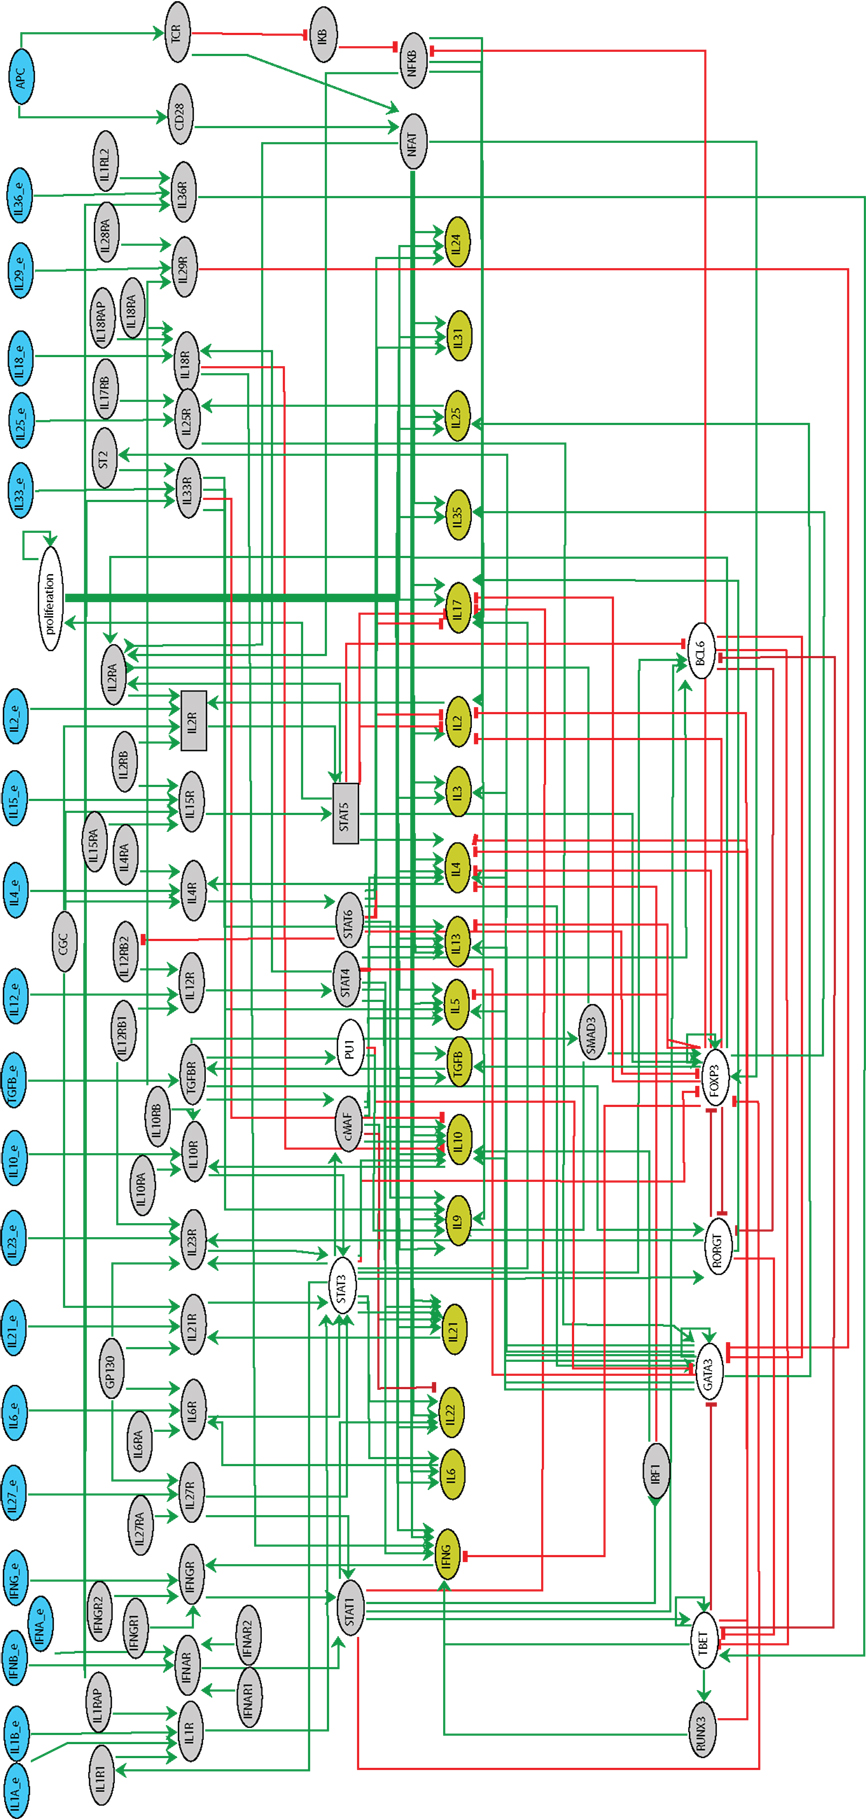
\includegraphics[scale=0.18,angle=-90]{images/th_differentiation.jpg}
\end{center}
\begin{center}
 {\tiny \color{darkgreen} [\citeatfb]}
\end{center}
\end{frame}



%mettre le tableau
\begin{frame}[c]
 \frametitle{Results of identification of bifurcations}
 

%mettre le tableau
\begin{table}[bt]
\renewcommand{\arraystretch}{1.3}

\centering
%table of result
\scalebox{0.8}{
\setlength{\tabcolsep}{2mm}
\begin{tabular}{|c|c||c|r||c|r||c|r|}
\hline
\multirow{2}{*}{Automata Network} 
& \multirow{2}{*}{Goal}
& \multicolumn{2}{c||}{M-C (NuSMV)}
& \multicolumn{2}{c||}{with \iIIIa}
& \multicolumn{2}{c|}{with \iIIIb}
\\
\cline{3-8}
&&$\card{t_b}$&Time&$\card{t_b}$&Time&$\card{t_b}$&Time
\\\hline

Lambda phage &  $\mathrm{CI}_2$ & $10$ & $0.1s$ & $6$ & $0.1s$ & $0$ & $0.2s$ 	
\\
$\card\anN=4\quad\card\anT=11$ &$\mathrm{Cro}_2$ & $3$ & $0.1s$ & $3$ & $0.1s$ & $2$ & $0.3s$ 	
\\ \hline 

EGF/TNF       & $\mathrm{NFkB}_0$ & $5$ & $0.2s$ & $4$ & $0.1s$ & $2$ & $0.1s$ 
\\

$\card\anN=28\quad\card\anT=55$ & $\mathrm{IKB}_1$ & $5$ & $0.2s$ & $3$ & $0.1s$ & $2$ & $0.1s$ 

\\ \hline

Th\_th17 & $\mathrm{RORGT}_1$ & $18$ & $48s$ & $9$ & $23s$ & $8$ & $26s$  
\\
$\card\anN=101\quad\card\anT=381$ & $\mathrm{BCL6}_1$ &$7$ & $26s$ &$5$ & $23s$ & $4$ & $24s$ 

\\ \hline

Th\_HTG & $\mathrm{BCL6}_1$ & \multicolumn{2}{c||}{\multirow{2}{*}{out-of-time}} & \multicolumn{2}{c||}{\multirow{2}{*}{out-of-time}} & $6$ & $61s$ 

\\

$\card\anN=101\quad\card\anT=381$ & $\mathrm{GATA3}_1$ &  \multicolumn{2}{c||}{} &\multicolumn{2}{c||}{}  & $7$ & $34s$ 

\\ \hline



\end{tabular}
}

%ordonner le tableau, M-C par model checking (numsv),
%OT : out of time
%garder deux The

%on peut en rater des bifurcations
% pour certaines applications où la taille est trop importante ce n'est pas possible de faire un calcul exact
% enlever pfx
 

%\label{tab:methodtest}
\end{table}

\begin{center} Implemented in ASP (Answer Set Programming) and solve with clingo 4.5.4.\end{center}
\end{frame}



\begin{comment}
\begin{table}[bt]
\small
\renewcommand{\arraystretch}{1.3}

\centering
%table of result

\setlength{\tabcolsep}{2mm}
\begin{tabular}{|c|c||r|c|r||c|r|}
\hline
\multirow{2}{*}{Automata Network} 
& \multirow{2}{*}{Goal}
& \multicolumn{3}{c||}{\iIIIa}
& \multicolumn{2}{c|}{\iIIIb}
\\
\cline{3-7}
&&$\card{\unf(s_0)}$&$\card{t_b}$&Time&$\card{t_b}$&Time
\\\hline

Lambda phage &  $\mathrm{CI}_2$ & \multirow{2}{*}{45} & $6$ & $0.14s$ & $0$ & $0.34s$ 
\\
$\card\anN=4\quad\card\anT=11$ &$\mathrm{Cro}_2$ & & $3$ & $0.15s$ & $2$ & $0.44s$ 
\\ \hline 

EGF/TNF  & $\mathrm{NFkB}_0$ & \multirow{2}{*}{52} & $4$ & $0.07s$ & $2$ & $0.15s$

\\

$\card\anN=28\quad\card\anT=55$ & $\mathrm{IKB}_1$ & & $3$ & $0.07s$ & $2$ & $0.13s$

\\ \hline


Th\_th1 & $\mathrm{BCL6}_1$ & \multirow{2}{*}{444} & $6$ & $19.6s$  & $5$ & $25.82s$

\\
$\card\anN=101\quad\card\anT=381$ & 
$\mathrm{TBET}_1$ &  & $5$ & $13.08s$  & $4$ & $26.4s$

\\ \hline


Th\_th2 & $\mathrm{GATA3}_0$ & \multirow{2}{*}{3264} & $7$ & $28.7s$  & $4$ & $27.5s$
\\
$\card\anN=101\quad\card\anT=381$ &
	$\mathrm{BCL6}_1$ & & $5$ & $28.4s$ & $4$ & $28.01s$

\\ \hline

Th\_th17 & $\mathrm{RORGT}_1$ &\multirow{2}{*}{2860} & $9$ & $23.9s$ & $8$ & $29.04s$  

\\
$\card\anN=101\quad\card\anT=381$ &

$\mathrm{BCL6}_1$ & &$5$ & $26.2s$ & $4$ & $26.64s$ 

\\ \hline

Th\_HTG & $\mathrm{BCL6}_1$ & \multirow{2}{*}{OT} & - & - & $6$ & $61.9s$

\\

$\card\anN=101\quad\card\anT=381$ &

$\mathrm{GATA3}_1$ & & - & - & $7$ & $34.16s$ 

\\ \hline


\end{tabular}
%\caption{
%Experimental results for the identification of bifurcations depending if \iIIIa or \iIIIb is used.
%Models Th\_th1, Th\_th2, Th\_th17, Th\_HTG are the same automata network but have different initial
%state.
%For each model, two different goals have been tested.
%$\card\anN$ is the number of automata, and $\card\anT$ the number of transitions;
%$\card{\inf(s_0)}$ is the size (number of events in the partial order structure) of the prefix of the unfolding from the initial state of the model;
%$\card{t_b}$ is the number of identified bifurcation transitions.
%Computation times have been obtained on an  Intel\textregistered{} Core\texttrademark{} i7-4600M
%2.90GHz CPU with 7.7GiB of RAM.
%OT indicates an out-of-time execution (more than one hour).}


\label{tab:methodtest}
\end{table}

\end{frame}

%%remettre le begin comment ici
The last experiment shows the limit of the exact analysis of the reachable state 
space: the computation of the prefix is not tractable on this model.
However, the alternative approach \iIIIb allows to identify bifurcation transitions in this large
model.
Following \secref{scheme}, \iIIIb always results in less bifurcations transitions than \iIIIa with
our models. It can be explained with the additional approximation for the reachability of $s_b$ from
$s_0$, using the notations of \secref{bifurcation}.
One can finally remark that when \iIIIa is tractable, \iIIIb shows a slightly slower solving
time, albeit of the same order of magnitude.
This suggest that checking if a state belongs to an unfolding is more efficient than checking 
its under-approximation.
Finally, because there exists to our knowledge no other method for identifying bifurcations, we
cannot compare our results with different methods, and in particular with an exact method in order
to appreciate the false negative rate obtained by the \iI-\iII-\iIIIa scheme.


\begin{frame}[c]
 \frametitle{Impact on probability}
 


\begin{center}
  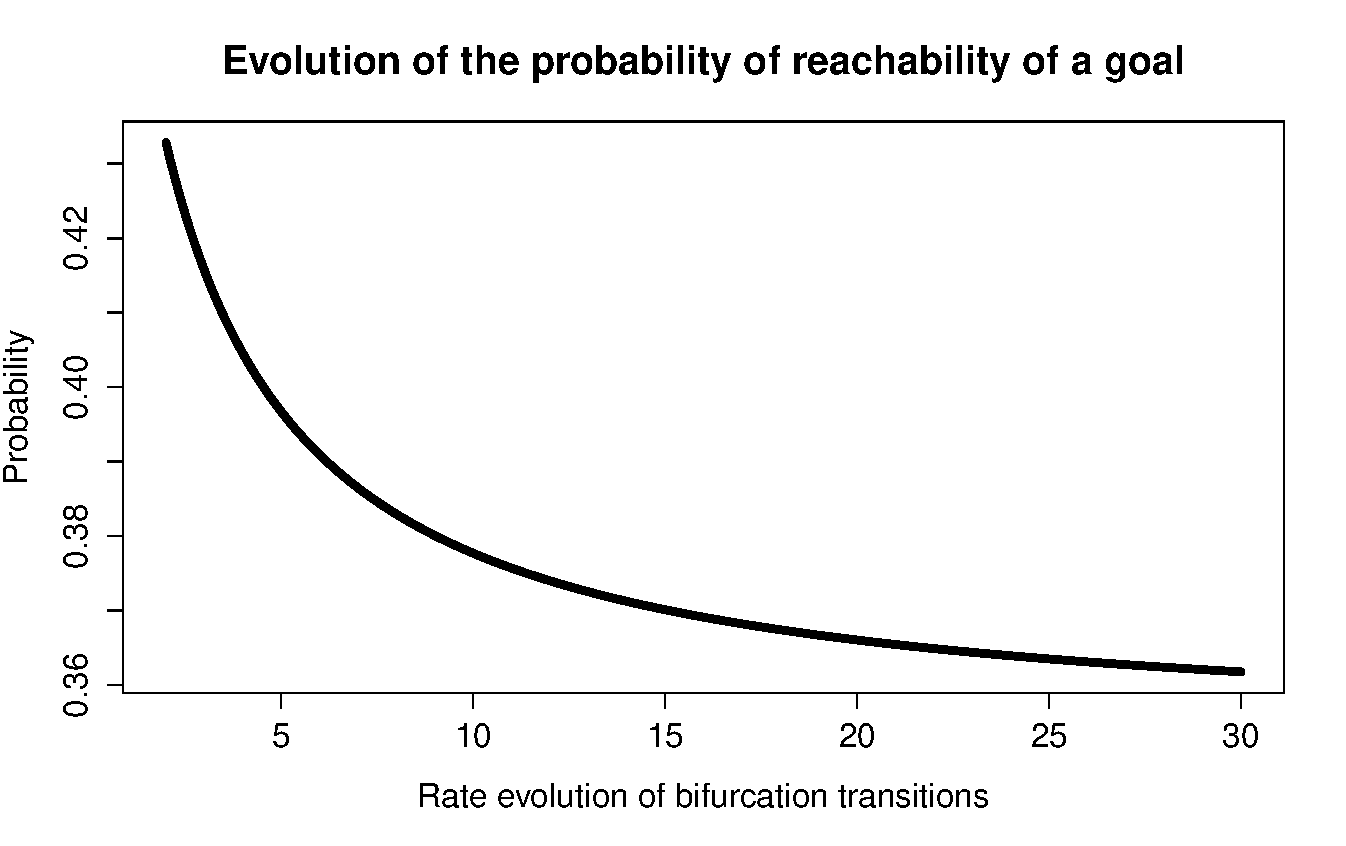
\includegraphics[scale=0.4]{images/prob_evol_new.pdf}
\end{center}
 

\begin{itemize}
 \item PRISM for simulation.
 \item A decrease of the probability of reach $CI=2$ in the lambda phage model from the initial state.
\end{itemize}
 
\end{frame}
\end{comment}



%%%%%%%    la conclusion
\section{Conclusions \& Perspectives}
% Performances et conclusion
\begin{frame}[c]
  \frametitle{Conclusions \& Perspectives}

%mots clés: large scale
%bien expliquer les résultats obtenus
 \textbf{Summary}
 \begin{itemize}
\item 
$$
\left\{
    \begin{array}{lcl}
        \mbox{AI (Artificial inteligence)} &\\  %rajouter un signe entre les deux
        \mbox{+} & $\Longrightarrow$ \mbox{\tval{formal approximation of bifurcations}} \\
        \mbox{AI (Abstract interpretation)} &
    \end{array}
\right.
$$ 
   \item Tractable on large networks (compared to model-checking)
   \item Under-approximation: some bifurcations are not returned.
   %\item Application on \tval{Phage lambda, EGF/TNF, Th\_differentiation} 
  \end{itemize}
\medskip
\textbf{Perspectives}
 \begin{itemize}
%parler d'améliorer les conditions initiales
  \item Over-approximation of bifurcations
  %\item Frame the number of attractors
  \item Use bifurcations for the analysis of probability 
  \item Applications for \tval{predicting targets for cellular reprogramming.}
  
 \end{itemize}
%\medskip

\end{frame}

%rajouter les slides du titre




%\begin{frame}
 \frametitle{Perspectives}
 
 \begin{block}{Formal verification of quantitative properties and key process (in progress)}
  \begin{itemize}
   \item Static analysis of quantitative properties of reachability in Asynchronous automata networks
   \item Logical verification and key processes detection
   \item Experimental validation of in silico hypotesis
   %\item Integrate de likelihood in the parameters estimation procedure.
  \end{itemize}

 \end{block}
 
 \begin{block}{Association rules and traces in automata networks}
  \begin{itemize}
   \item Association rules for discovering interesting relations between local states. 
   \item Experimental validation of in silico hypotesis
  \end{itemize}

 \end{block}
 
\end{frame}

\begin{frame}
Vielen Dank für Ihre Aufmerksamkeit!!!
\end{frame}


\begin{frame}[plain,label=title]

% Cadre de titre
\begin{center}
\vspace{1cm}
\setbeamercolor{postit}{fg=black,bg=colortitle}
\begin{beamercolorbox}[sep=0.5em]{postit}
\centering
\Large
\textbf{%
{\normalsize\theconference{}}\\~\\%
\inserttitle
}
\end{beamercolorbox}

% Auteurs et instituts
% Auteurs et instituts
\par
\medskip
\normalsize
Louis Fippo Fitime$^{1}$
\footnotesize

\texttt{louis.fippo-fitime@irccyn.ec-nantes.fr}

%\url{http://www.irccyn.ec-nantes.fr/~folschet/}

\normalsize
\bigskip
\textbf{Joint work with:} \\  Olivier Roux$^1$, Carito Guziolowski$^1$ and Lo\"ic Paulev\'e$^2$

\medskip
\footnotesize
$^1$ MeForBio / IRCCyN / École Centrale de Nantes (Nantes, France)\\
$^2$ Bioinfo / LRI / CNRS (Paris, France)

\texttt{olivier.roux@irccyn.ec-nantes.fr}

\texttt{carito.guziolowski@irccyn.ec-nantes.fr}

\texttt{loic.pauleve@lri.fr}

\end{center}
Thank you for your attention!
\end{frame}




%%%%%% appendix and bibliographie
%\appendix
%\section[x]{Bibliography}
%% Bibliographie

\begin{frame}[c]
  \frametitle{Bibliography}

\footnotesize
\setlength{\parindent}{-1em}
\setlength{\parskip}{0.5em}
~

\vfill
%\tcite{Paulevé11} Loïc Paulevé. PhD thesis: \textit{Modélisation, Simulation et Vérification des Grands Réseaux de Régulation Biologique}, October 2011, Nantes, France

\tcite{Paulev\'e et al. 2010} Loïc Paulevé, Morgan Magnin, and Olivier Roux. \textit{Tuning Temporal Features within the Stochastic $\pi$-Calculus}. IEEE Transactions on Software Engineering, 37(6):858-871, 2011.

%\tcite{PRM10-TCSB} Loïc Paulevé, Morgan Magnin, and Olivier Roux. \textit{Refining dynamics of gene regulatory networks in a stochastic $\pi$-calculus framework}. In Corrado Priami, Ralph-Johan Back, Ion Petre, and Erik de Vink, editors: Transactions on Computational Systems Biology XIII, volume 6575 of Lecture Notes in Computer Science, 171-191. Springer Berlin/Heidelberg, 2011.

\tcite{Paulev\'e et al. 2012} Loïc Paulevé, Morgan Magnin, and Olivier Roux. \textit{Static analysis of biological regulatory networks dynamics using abstract interpretation}. Mathematical Structures in Computer Science, in press, 2012.

%\tcite{PR10-CRAS} Loïc Paulevé and Adrien Richard. \textit{Topological Fixed Points in Boolean Networks}. Comptes Rendus de l'Académie des Sciences - Series I - Mathematics, 348(15-16):825 - 828, 2010.

\tcite{Richard et al. 2008} Adrien Richard, Jean-Paul Comet, and Gilles Bernot. \textit{R. Thomas' logical method}, 2008. Invited at Tutorials on modelling methods and tools: Modelling a genetic switch and Metabolic Networks, Spring School on Modelling Complex Biological Systems in the Context of Genomics.

%\tcite{CMSB12} Maxime Folschette, Loïc Paulevé, Katsumi Inoue, Morgan Magnin, and Olivier Roux. \textit{Concretizing the Process Hitting into Biological Regulatory Networks}. In: Computational Methods in Systems Biology, Springer, 2012.




\tcite{Ahmad et al. 2008}
Jamil Ahmad, Olivier Roux, Gilles Bernot, Jean-Paul Comet, and Adrien Richard.
\textit{Analysing formal models of genetic regulatory networks with delays.}
 International Journal of Bioinformatics Research and
  Applications (IJBRA), 4(3):240--262, 2008.

\tcite{Batt et al. 2007}
Gr{\'e}gory Batt, Ramzi~Ben Salah, and Oded Maler.
 \textit{On timed models of gene networks.}
 Springer, 2007.

\tcite{Gardner et al. 2003}
Timothy~S Gardner, Diego Di~Bernardo, David Lorenz, and James~J Collins.
 \textit{Inferring genetic networks and identifying compound mode of action
  via expression profiling.}
  Science, 301(5629):102--105, 2003.

\tcite{Guziolowski et al. 2012}
Carito Guziolowski, Aristotelis Kittas, Florian Dittmann, and Niels Grabe.
\textit{ Automatic generation of causal networks linking growth factor stimuli
  to functional cell state changes.}
 FEBS Journal, 279(18):3462--3474, 2012.

\tcite{Heiner et al. 2008}
Monika Heiner, David Gilbert, and Robin Donaldson.
 \textit{Petri nets for systems and synthetic biology.}
 Formal methods for computational systems biology, pages
  215--264. Springer, 2008.

\tcite{Mac Namara et al. 2012}
Aidan MacNamara, Camille Terfve, David Henriques, Beatriz~Pe{\~n}alver
  Bernab{\'e}, and Julio Saez-Rodriguez.
 \textit{State--time spectrum of signal transduction logic models.}
 Physical Biology, 9(4):045003, 2012.


\vfill
\Large
\begin{flushright}
  \tval{Thank you}\hspace{1cm}~
\end{flushright}
\vfill

~

\end{frame}



%%%%%% section annexe 

\begin{comment}
plan pour la presentation de ma thèse

-introduction

-integration des données

-analyse statitique des propriétés quantitatives
  
  *probability in CTMC
  *

-analyse statique des bifurcations

-implementation

-biological applications



\end{comment}




\end{document}
